%%%%%%%%%%%%%%%%%%%%%%%%%%%%%%%%%%%%%%%%%%%%%%%%%%%%%%%%%%%%%%%%%%%%%%%%%%%%%%%%
%%%%%%%%%%%%%%%%%%   Vorlage für eine Abschlussarbeit   %%%%%%%%%%%%%%%%%%%%%%%%
%%%%%%%%%%%%%%%%%%%%%%%%%%%%%%%%%%%%%%%%%%%%%%%%%%%%%%%%%%%%%%%%%%%%%%%%%%%%%%%%

% Erstellt von Maximilian Nöthe, <maximilian.noethe@tu-dortmund.de>
% ausgelegt für lualatex und Biblatex mit biber

% Kompilieren mit
% latexmk --lualatex --output-directory=build thesis.tex
% oder einfach mit:
% make

\documentclass[
  tucolor,       % remove for less green,
  BCOR=12mm,     % 12mm binding corrections, adjust to fit your binding
  parskip=half,  % new paragraphs start with half line vertical space
  open=any,      % chapters start on both odd and even pages
  cleardoublepage=plain,  % no header/footer on blank pages
]{tudothesis}

% Package for insertion of line numbers
\usepackage{lineno}

% Warning, if another latex run is needed
\usepackage[aux]{rerunfilecheck}

% just list chapters and sections in the toc, not subsections or smaller
\setcounter{tocdepth}{1}

%------------------------------------------------------------------------------
%------------------------------ Fonts, Unicode, Language ----------------------
%------------------------------------------------------------------------------
\usepackage{fontspec}
\defaultfontfeatures{Ligatures=TeX}  % -- becomes en-dash etc.

% load all used languages
% and set the main language of this thesis
% use this if this thesis is written in German:
%\usepackage[main=ngerman, english]{babel}
% use this if this thesis is written in English:
\usepackage[ngerman, english]{babel}

% intelligent quotation marks, language and nesting sensitive
\usepackage[autostyle]{csquotes}

% microtypographical features, makes the text look nicer on the small scale
\usepackage{microtype}

%------------------------------------------------------------------------------
%------------------------ Math Packages and settings --------------------------
%------------------------------------------------------------------------------

\usepackage{amsmath}
\usepackage{amssymb}
\usepackage{mathtools}
\usepackage{ifthenx}
%%% $Id: lhcb-symbols-def.tex 124462 2018-11-07 12:32:50Z pkoppenb $
%%% ======================================================================
%%% Purpose: Standard LHCb aliases
%%% Author: Originally Ulrik Egede, adapted by Tomasz Skwarnicki for templates,
%%% rewritten by Chris Parkes
%%% Maintainer : Ulrik Egede (2010 - 2012)
%%% Maintainer : Rolf Oldeman (2012 - 2014)
%%% Maintainer : Patrick Koppenburg (2018--2020)
%%% =======================================================================

%%% To use this file outside the normal LHCb document environment, the
%%% following should be added in a preamble (before \begin{document}
%%%
%%%\usepackage{ifthen}
%%%\newboolean{uprightparticles}
%%%\setboolean{uprightparticles}{false} %Set true for upright particle symbols
\usepackage{xspace}
\usepackage{upgreek}

\newcommand{\offsetoverline}[2][0.1em]{\kern #1\overline{\kern -#1 #2}}%

%%%%%%%%%%%%%%%%%%%%%%%%%%%%%%%%%%%%%%%%%%%%%%%%%%%%%%%%%%%%
%%%
%%% The following is to ensure that the template automatically can process
%%% this file.
%%%
%%% Add comments with at least three %%% preceding.
%%% Add new sections with one % preceding
%%% Add new subsections with two %% preceding
%%%
%%% For upper greek letters, Xires and Xiresbar will be the particles without the charge
%%% States with charge are called Xiz and Xim
%%%
%%%%%%%%%%%%%%%%%%%%%%%%%%%%%%%%%%%%%%%%%%%%%%%%%%%%%%%%%%%%

%%%%%%%%%%%%%
% Experiments
%%%%%%%%%%%%%
\def\lhcb   {\mbox{LHCb}\xspace}
\def\atlas  {\mbox{ATLAS}\xspace}
\def\cms    {\mbox{CMS}\xspace}
\def\alice  {\mbox{ALICE}\xspace}
\def\babar  {\mbox{BaBar}\xspace}
\def\belle  {\mbox{Belle}\xspace}
\def\belletwo {\mbox{Belle~II}\xspace}
\def\besiii {\mbox{BESIII}\xspace}
\def\cleo   {\mbox{CLEO}\xspace}
\def\cdf    {\mbox{CDF}\xspace}
\def\dzero  {\mbox{D0}\xspace}
\def\aleph  {\mbox{ALEPH}\xspace}
\def\delphi {\mbox{DELPHI}\xspace}
\def\opal   {\mbox{OPAL}\xspace}
\def\lthree {\mbox{L3}\xspace}
\def\sld    {\mbox{SLD}\xspace}
%%%\def\argus  {\mbox{ARGUS}\xspace}
%%%\def\uaone  {\mbox{UA1}\xspace}
%%%\def\uatwo  {\mbox{UA2}\xspace}
%%%\def\ux85 {\mbox{UX85}\xspace}
\def\cern {\mbox{CERN}\xspace}
\def\lhc    {\mbox{LHC}\xspace}
\def\lep    {\mbox{LEP}\xspace}
\def\tevatron {Tevatron\xspace}
\def\bfactories {\mbox{\B Factories}\xspace}
\def\bfactory   {\mbox{\B Factory}\xspace}
\def\upgradeone {\mbox{Upgrade~I}\xspace}
\def\upgradetwo {\mbox{Upgrade~II}\xspace}

%% LHCb sub-detectors and sub-systems

%%%\def\pu     {PU\xspace}
\def\velo   {VELO\xspace}
\def\rich   {RICH\xspace}
\def\richone {RICH1\xspace}
\def\richtwo {RICH2\xspace}
\def\ttracker {TT\xspace}
\def\intr   {IT\xspace}
\def\st     {ST\xspace}
\def\ot     {OT\xspace}
\def\herschel {\mbox{\textsc{HeRSCheL}}\xspace}
%%%\def\Tone   {T1\xspace}
%%%\def\Ttwo   {T2\xspace}
%%%\def\Tthree {T3\xspace}
%%%\def\Mone   {M1\xspace}
%%%\def\Mtwo   {M2\xspace}
%%%\def\Mthree {M3\xspace}
%%%\def\Mfour  {M4\xspace}
%%%\def\Mfive  {M5\xspace}
\def\spd    {SPD\xspace}
\def\presh  {PS\xspace}
\def\ecal   {ECAL\xspace}
\def\hcal   {HCAL\xspace}
%%%\def\bcm    {BCM\xspace}
\def\MagUp {\mbox{\em Mag\kern -0.05em Up}\xspace}
\def\MagDown {\mbox{\em MagDown}\xspace}

\def\ode    {ODE\xspace}
\def\daq    {DAQ\xspace}
\def\tfc    {TFC\xspace}
\def\ecs    {ECS\xspace}
\def\lone   {L0\xspace}
\def\hlt    {HLT\xspace}
\def\hltone {HLT1\xspace}
\def\hlttwo {HLT2\xspace}

%%% Upright (not slanted) Particles

%\ifthenelse{\boolean{uprightparticles}}%
%{\def\Palpha      {\ensuremath{\upalpha}\xspace}
% \def\Pbeta       {\ensuremath{\upbeta}\xspace}
% \def\Pgamma      {\ensuremath{\upgamma}\xspace}
% \def\Pdelta      {\ensuremath{\updelta}\xspace}
% \def\Pepsilon    {\ensuremath{\upepsilon}\xspace}
% \def\Pvarepsilon {\ensuremath{\upvarepsilon}\xspace}
% \def\Pzeta       {\ensuremath{\upzeta}\xspace}
% \def\Peta        {\ensuremath{\upeta}\xspace}
% \def\Ptheta      {\ensuremath{\uptheta}\xspace}
% \def\Pvartheta   {\ensuremath{\upvartheta}\xspace}
% \def\Piota       {\ensuremath{\upiota}\xspace}
% \def\Pkappa      {\ensuremath{\upkappa}\xspace}
% \def\Plambda     {\ensuremath{\uplambda}\xspace}
% \def\Pmu         {\ensuremath{\upmu}\xspace}
% \def\Pnu         {\ensuremath{\upnu}\xspace}
% \def\Pxi         {\ensuremath{\upxi}\xspace}
% \def\Ppi         {\ensuremath{\uppi}\xspace}
% \def\Pvarpi      {\ensuremath{\upvarpi}\xspace}
% \def\Prho        {\ensuremath{\uprho}\xspace}
% \def\Pvarrho     {\ensuremath{\upvarrho}\xspace}
% \def\Ptau        {\ensuremath{\uptau}\xspace}
% \def\Pupsilon    {\ensuremath{\upupsilon}\xspace}
% \def\Pphi        {\ensuremath{\upphi}\xspace}
% \def\Pvarphi     {\ensuremath{\upvarphi}\xspace}
% \def\Pchi        {\ensuremath{\upchi}\xspace}
% \def\Ppsi        {\ensuremath{\uppsi}\xspace}
% \def\Pomega      {\ensuremath{\upomega}\xspace}
%
% \def\PDelta      {\ensuremath{\Delta}\xspace}
% \def\PXi         {\ensuremath{\Xi}\xspace}
% \def\PLambda     {\ensuremath{\Lambda}\xspace}
% \def\PSigma      {\ensuremath{\Sigma}\xspace}
% \def\POmega      {\ensuremath{\Omega}\xspace}
% \def\PUpsilon    {\ensuremath{\Upsilon}\xspace}
%
% \def\PA      {\ensuremath{\mathrm{A}}\xspace}
% \def\PB      {\ensuremath{\mathrm{B}}\xspace}
% \def\PC      {\ensuremath{\mathrm{C}}\xspace}
% \def\PD      {\ensuremath{\mathrm{D}}\xspace}
% \def\PE      {\ensuremath{\mathrm{E}}\xspace}
% \def\PF      {\ensuremath{\mathrm{F}}\xspace}
% \def\PG      {\ensuremath{\mathrm{G}}\xspace}
% \def\PH      {\ensuremath{\mathrm{H}}\xspace}
% \def\PI      {\ensuremath{\mathrm{I}}\xspace}
% \def\PJ      {\ensuremath{\mathrm{J}}\xspace}
% \def\PK      {\ensuremath{\mathrm{K}}\xspace}
% \def\PL      {\ensuremath{\mathrm{L}}\xspace}
% \def\PM      {\ensuremath{\mathrm{M}}\xspace}
% \def\PN      {\ensuremath{\mathrm{N}}\xspace}
% \def\PO      {\ensuremath{\mathrm{O}}\xspace}
% \def\PP      {\ensuremath{\mathrm{P}}\xspace}
% \def\PQ      {\ensuremath{\mathrm{Q}}\xspace}
% \def\PR      {\ensuremath{\mathrm{R}}\xspace}
% \def\PS      {\ensuremath{\mathrm{S}}\xspace}
% \def\PT      {\ensuremath{\mathrm{T}}\xspace}
% \def\PU      {\ensuremath{\mathrm{U}}\xspace}
% \def\PV      {\ensuremath{\mathrm{V}}\xspace}
% \def\PW      {\ensuremath{\mathrm{W}}\xspace}
% \def\PX      {\ensuremath{\mathrm{X}}\xspace}
% \def\PY      {\ensuremath{\mathrm{Y}}\xspace}
% \def\PZ      {\ensuremath{\mathrm{Z}}\xspace}
% \def\Pa      {\ensuremath{\mathrm{a}}\xspace}
% \def\Pb      {\ensuremath{\mathrm{b}}\xspace}
% \def\Pc      {\ensuremath{\mathrm{c}}\xspace}
% \def\Pd      {\ensuremath{\mathrm{d}}\xspace}
% \def\Pe      {\ensuremath{\mathrm{e}}\xspace}
% \def\Pf      {\ensuremath{\mathrm{f}}\xspace}
% \def\Pg      {\ensuremath{\mathrm{g}}\xspace}
% \def\Ph      {\ensuremath{\mathrm{h}}\xspace}
% \def\Pi      {\ensuremath{\mathrm{i}}\xspace}
% \def\Pj      {\ensuremath{\mathrm{j}}\xspace}
% \def\Pk      {\ensuremath{\mathrm{k}}\xspace}
% \def\Pl      {\ensuremath{\mathrm{l}}\xspace}
% \def\Pm      {\ensuremath{\mathrm{m}}\xspace}
% \def\Pn      {\ensuremath{\mathrm{n}}\xspace}
% \def\Po      {\ensuremath{\mathrm{o}}\xspace}
% \def\Pp      {\ensuremath{\mathrm{p}}\xspace}
% \def\Pq      {\ensuremath{\mathrm{q}}\xspace}
% \def\Pr      {\ensuremath{\mathrm{r}}\xspace}
% \def\Ps      {\ensuremath{\mathrm{s}}\xspace}
% \def\Pt      {\ensuremath{\mathrm{t}}\xspace}
% \def\Pu      {\ensuremath{\mathrm{u}}\xspace}
% \def\Pv      {\ensuremath{\mathrm{v}}\xspace}
% \def\Pw      {\ensuremath{\mathrm{w}}\xspace}
% \def\Px      {\ensuremath{\mathrm{x}}\xspace}
% \def\Py      {\ensuremath{\mathrm{y}}\xspace}
% \def\Pz      {\ensuremath{\mathrm{z}}\xspace}
%}
\def\Palpha      {\ensuremath{\alpha}\xspace}
 \def\Pbeta       {\ensuremath{\beta}\xspace}
 \def\Pgamma      {\ensuremath{\gamma}\xspace}
 \def\Pdelta      {\ensuremath{\delta}\xspace}
 \def\Pepsilon    {\ensuremath{\epsilon}\xspace}
 \def\Pvarepsilon {\ensuremath{\varepsilon}\xspace}
 \def\Pzeta       {\ensuremath{\zeta}\xspace}
 \def\Peta        {\ensuremath{\eta}\xspace}
 \def\Ptheta      {\ensuremath{\theta}\xspace}
 \def\Pvartheta   {\ensuremath{\vartheta}\xspace}
 \def\Piota       {\ensuremath{\iota}\xspace}
 \def\Pkappa      {\ensuremath{\kappa}\xspace}
 \def\Plambda     {\ensuremath{\lambda}\xspace}
 \def\Pmu         {\ensuremath{\mu}\xspace}
 \def\Pnu         {\ensuremath{\nu}\xspace}
 \def\Pxi         {\ensuremath{\xi}\xspace}
 \def\Ppi         {\ensuremath{\pi}\xspace}
 \def\Pvarpi      {\ensuremath{\varpi}\xspace}
 \def\Prho        {\ensuremath{\rho}\xspace}
 \def\Pvarrho     {\ensuremath{\varrho}\xspace}
 \def\Ptau        {\ensuremath{\tau}\xspace}
 \def\Pupsilon    {\ensuremath{\upsilon}\xspace}
 \def\Pphi        {\ensuremath{\phi}\xspace}
 \def\Pvarphi     {\ensuremath{\varphi}\xspace}
 \def\Pchi        {\ensuremath{\chi}\xspace}
 \def\Ppsi        {\ensuremath{\psi}\xspace}
 \def\Pomega      {\ensuremath{\omega}\xspace}
 \mathchardef\PDelta="7101
 \mathchardef\PXi="7104
 \mathchardef\PLambda="7103
 \mathchardef\PSigma="7106
 \mathchardef\POmega="710A
 \mathchardef\PUpsilon="7107
 \def\PA      {\ensuremath{A}\xspace}
 \def\PB      {\ensuremath{B}\xspace}
 \def\PC      {\ensuremath{C}\xspace}
 \def\PD      {\ensuremath{D}\xspace}
 \def\PE      {\ensuremath{E}\xspace}
 \def\PF      {\ensuremath{F}\xspace}
 \def\PG      {\ensuremath{G}\xspace}
 \def\PH      {\ensuremath{H}\xspace}
 \def\PI      {\ensuremath{I}\xspace}
 \def\PJ      {\ensuremath{J}\xspace}
 \def\PK      {\ensuremath{K}\xspace}
 \def\PL      {\ensuremath{L}\xspace}
 \def\PM      {\ensuremath{M}\xspace}
 \def\PN      {\ensuremath{N}\xspace}
 \def\PO      {\ensuremath{O}\xspace}
 \def\PP      {\ensuremath{P}\xspace}
 \def\PQ      {\ensuremath{Q}\xspace}
 \def\PR      {\ensuremath{R}\xspace}
 \def\PS      {\ensuremath{S}\xspace}
 \def\PT      {\ensuremath{T}\xspace}
 \def\PU      {\ensuremath{U}\xspace}
 \def\PV      {\ensuremath{V}\xspace}
 \def\PW      {\ensuremath{W}\xspace}
 \def\PX      {\ensuremath{X}\xspace}
 \def\PY      {\ensuremath{Y}\xspace}
 \def\PZ      {\ensuremath{Z}\xspace}
 \def\Pa      {\ensuremath{a}\xspace}
 \def\Pb      {\ensuremath{b}\xspace}
 \def\Pc      {\ensuremath{c}\xspace}
 \def\Pd      {\ensuremath{d}\xspace}
 \def\Pe      {\ensuremath{e}\xspace}
 \def\Pf      {\ensuremath{f}\xspace}
 \def\Pg      {\ensuremath{g}\xspace}
 \def\Ph      {\ensuremath{h}\xspace}
 \def\Pi      {\ensuremath{i}\xspace}
 \def\Pj      {\ensuremath{j}\xspace}
 \def\Pk      {\ensuremath{k}\xspace}
 \def\Pl      {\ensuremath{l}\xspace}
 \def\Pm      {\ensuremath{m}\xspace}
 \def\Pn      {\ensuremath{n}\xspace}
 \def\Po      {\ensuremath{o}\xspace}
 \def\Pp      {\ensuremath{p}\xspace}
 \def\Pq      {\ensuremath{q}\xspace}
 \def\Pr      {\ensuremath{r}\xspace}
 \def\Ps      {\ensuremath{s}\xspace}
 \def\Pt      {\ensuremath{t}\xspace}
 \def\Pu      {\ensuremath{u}\xspace}
 \def\Pv      {\ensuremath{v}\xspace}
 \def\Pw      {\ensuremath{w}\xspace}
 \def\Px      {\ensuremath{x}\xspace}
 \def\Py      {\ensuremath{y}\xspace}
 \def\Pz      {\ensuremath{z}\xspace}


%%%%%%%%%%%%%%%%%%%%%%%%%%%%%%%%%%%%%%%%%%%%%%%
% Particles
\makeatletter
\ifcase \@ptsize \relax% 10pt
  \newcommand{\miniscule}{\@setfontsize\miniscule{4}{5}}% \tiny: 5/6
\or% 11pt
  \newcommand{\miniscule}{\@setfontsize\miniscule{5}{6}}% \tiny: 6/7
\or% 12pt
  \newcommand{\miniscule}{\@setfontsize\miniscule{5}{6}}% \tiny: 6/7
\fi
\makeatother


\DeclareRobustCommand{\optbar}[1]{\shortstack{{\miniscule (\rule[.5ex]{1.25em}{.18mm})}
  \\ [-.7ex] $#1$}}


%% Leptons

\let\emi\en
\def\electron   {{\ensuremath{\Pe}}\xspace}
\def\en         {{\ensuremath{\Pe^-}}\xspace}   % electron negative (\em is taken)
\def\ep         {{\ensuremath{\Pe^+}}\xspace}
\def\epm        {{\ensuremath{\Pe^\pm}}\xspace}
\def\emp        {{\ensuremath{\Pe^\mp}}\xspace}
\def\epem       {{\ensuremath{\Pe^+\Pe^-}}\xspace}
%%%\def\ee         {\ensuremath{\Pe^-\Pe^-}\xspace}

\def\muon       {{\ensuremath{\Pmu}}\xspace}
\def\mup        {{\ensuremath{\Pmu^+}}\xspace}
\def\mun        {{\ensuremath{\Pmu^-}}\xspace} % muon negative (\mum is taken)
\def\mupm       {{\ensuremath{\Pmu^\pm}}\xspace}
\def\mump       {{\ensuremath{\Pmu^\mp}}\xspace}
\def\mumu       {{\ensuremath{\Pmu^+\Pmu^-}}\xspace}

\def\tauon      {{\ensuremath{\Ptau}}\xspace}
\def\taup       {{\ensuremath{\Ptau^+}}\xspace}
\def\taum       {{\ensuremath{\Ptau^-}}\xspace}
\def\taupm      {{\ensuremath{\Ptau^\pm}}\xspace}
\def\taump      {{\ensuremath{\Ptau^\mp}}\xspace}
\def\tautau     {{\ensuremath{\Ptau^+\Ptau^-}}\xspace}

\def\lepton     {{\ensuremath{\ell}}\xspace}
\def\ellm       {{\ensuremath{\ell^-}}\xspace}
\def\ellp       {{\ensuremath{\ell^+}}\xspace}
\def\ellell     {\ensuremath{\ell^+ \ell^-}\xspace}

\def\neu        {{\ensuremath{\Pnu}}\xspace}
\def\neub       {{\ensuremath{\overline{\Pnu}}}\xspace}
%%%\def\nuenueb    {\ensuremath{\neu\neub}\xspace}
\def\neue       {{\ensuremath{\neu_e}}\xspace}
\def\neueb      {{\ensuremath{\neub_e}}\xspace}
%%%\def\neueneueb  {\ensuremath{\neue\neueb}\xspace}
\def\neum       {{\ensuremath{\neu_\mu}}\xspace}
\def\neumb      {{\ensuremath{\neub_\mu}}\xspace}
%%%\def\neumneumb  {\ensuremath{\neum\neumb}\xspace}
\def\neut       {{\ensuremath{\neu_\tau}}\xspace}
\def\neutb      {{\ensuremath{\neub_\tau}}\xspace}
%%%\def\neutneutb  {\ensuremath{\neut\neutb}\xspace}
\def\neul       {{\ensuremath{\neu_\ell}}\xspace}
\def\neulb      {{\ensuremath{\neub_\ell}}\xspace}
%%%\def\neulneulb  {\ensuremath{\neul\neulb}\xspace}

%% Gauge bosons and scalars

\def\g      {{\ensuremath{\Pgamma}}\xspace}
\def\H      {{\ensuremath{\PH^0}}\xspace}
\def\Hp     {{\ensuremath{\PH^+}}\xspace}
\def\Hm     {{\ensuremath{\PH^-}}\xspace}
\def\Hpm    {{\ensuremath{\PH^\pm}}\xspace}
\def\W      {{\ensuremath{\PW}}\xspace}
\def\Wp     {{\ensuremath{\PW^+}}\xspace}
\def\Wm     {{\ensuremath{\PW^-}}\xspace}
\def\Wpm    {{\ensuremath{\PW^\pm}}\xspace}
\def\Z      {{\ensuremath{\PZ}}\xspace}

%% Quarks

\def\quark     {{\ensuremath{\Pq}}\xspace}
\def\quarkbar  {{\ensuremath{\overline \quark}}\xspace}
\def\qqbar     {{\ensuremath{\quark\quarkbar}}\xspace}
\def\uquark    {{\ensuremath{\Pu}}\xspace}
\def\uquarkbar {{\ensuremath{\overline \uquark}}\xspace}
\def\uubar     {{\ensuremath{\uquark\uquarkbar}}\xspace}
\def\dquark    {{\ensuremath{\Pd}}\xspace}
\def\dquarkbar {{\ensuremath{\overline \dquark}}\xspace}
\def\ddbar     {{\ensuremath{\dquark\dquarkbar}}\xspace}
\def\squark    {{\ensuremath{\Ps}}\xspace}
\def\squarkbar {{\ensuremath{\overline \squark}}\xspace}
\def\ssbar     {{\ensuremath{\squark\squarkbar}}\xspace}
\def\cquark    {{\ensuremath{\Pc}}\xspace}
\def\cquarkbar {{\ensuremath{\overline \cquark}}\xspace}
\def\ccbar     {{\ensuremath{\cquark\cquarkbar}}\xspace}
\def\bquark    {{\ensuremath{\Pb}}\xspace}
\def\bquarkbar {{\ensuremath{\overline \bquark}}\xspace}
\def\bbbar     {{\ensuremath{\bquark\bquarkbar}}\xspace}
\def\tquark    {{\ensuremath{\Pt}}\xspace}
\def\tquarkbar {{\ensuremath{\overline \tquark}}\xspace}
\def\ttbar     {{\ensuremath{\tquark\tquarkbar}}\xspace}

%% Light mesons

\def\hadron {{\ensuremath{\Ph}}\xspace}
\def\pion   {{\ensuremath{\Ppi}}\xspace}
\def\piz    {{\ensuremath{\pion^0}}\xspace}
\def\pip    {{\ensuremath{\pion^+}}\xspace}
\def\pim    {{\ensuremath{\pion^-}}\xspace}
\def\pipm   {{\ensuremath{\pion^\pm}}\xspace}
\def\pimp   {{\ensuremath{\pion^\mp}}\xspace}

\def\rhomeson {{\ensuremath{\Prho}}\xspace}
\def\rhoz     {{\ensuremath{\rhomeson^0}}\xspace}
\def\rhop     {{\ensuremath{\rhomeson^+}}\xspace}
\def\rhom     {{\ensuremath{\rhomeson^-}}\xspace}
\def\rhopm    {{\ensuremath{\rhomeson^\pm}}\xspace}
\def\rhomp    {{\ensuremath{\rhomeson^\mp}}\xspace}

\def\kaon    {{\ensuremath{\PK}}\xspace}
%%% do NOT use ensuremath here, and keep indent
  \def\Kbar    {{\kern 0.2em\overline{\kern -0.2em \PK}{}}\xspace}
\def\Kb      {{\ensuremath{\Kbar}}\xspace}
\def\KorKbar {\kern 0.18em\optbar{\kern -0.18em K}{}\xspace}
\def\Kz      {{\ensuremath{\kaon^0}}\xspace}
\def\Kzb     {{\ensuremath{\Kbar{}^0}}\xspace}
\def\Kp      {{\ensuremath{\kaon^+}}\xspace}
\def\Km      {{\ensuremath{\kaon^-}}\xspace}
\def\Kpm     {{\ensuremath{\kaon^\pm}}\xspace}
\def\Kmp     {{\ensuremath{\kaon^\mp}}\xspace}
\def\KS      {{\ensuremath{\kaon^0_{\mathrm{S}}}}\xspace}
\def\KL      {{\ensuremath{\kaon^0_{\mathrm{L}}}}\xspace}
\def\Kstarz  {{\ensuremath{\kaon^{*0}}}\xspace}
\def\Kstarzb {{\ensuremath{\Kbar{}^{*0}}}\xspace}
\def\Kstar   {{\ensuremath{\kaon^*}}\xspace}
\def\Kstarb  {{\ensuremath{\Kbar{}^*}}\xspace}
\def\Kstarp  {{\ensuremath{\kaon^{*+}}}\xspace}
\def\Kstarm  {{\ensuremath{\kaon^{*-}}}\xspace}
\def\Kstarpm {{\ensuremath{\kaon^{*\pm}}}\xspace}
\def\Kstarmp {{\ensuremath{\kaon^{*\mp}}}\xspace}
\def\KorKbarz {\ensuremath{\KorKbar^0}\xspace}

\newcommand{\etaz}{\ensuremath{\Peta}\xspace}
\newcommand{\etapr}{\ensuremath{\Peta^{\prime}}\xspace}
\newcommand{\phiz}{\ensuremath{\Pphi}\xspace}
\newcommand{\omegaz}{\ensuremath{\Pomega}\xspace}

%% Charmed mesons

%%% do NOT use ensuremath here (and keep indent)
  \def\Dbar    {{\kern 0.2em\overline{\kern -0.2em \PD}{}}\xspace}
\def\D       {{\ensuremath{\PD}}\xspace}
\def\Db      {{\ensuremath{\Dbar}}\xspace}
\def\DorDbar {\kern 0.18em\optbar{\kern -0.18em D}{}\xspace}
\def\Dz      {{\ensuremath{\D^0}}\xspace}
\def\Dzb     {{\ensuremath{\Dbar{}^0}}\xspace}
\def\Dp      {{\ensuremath{\D^+}}\xspace}
\def\Dm      {{\ensuremath{\D^-}}\xspace}
\def\Dpm     {{\ensuremath{\D^\pm}}\xspace}
\def\Dmp     {{\ensuremath{\D^\mp}}\xspace}
\def\Dstar   {{\ensuremath{\D^*}}\xspace}
\def\Dstarb  {{\ensuremath{\Dbar{}^*}}\xspace}
\def\Dstarz  {{\ensuremath{\D^{*0}}}\xspace}
\def\Dstarzb {{\ensuremath{\Dbar{}^{*0}}}\xspace}
\def\theDstarz{{\ensuremath{\D^{*}(2007)^{0}}}\xspace}
\def\theDstarzb{{\ensuremath{\Dbar^{*}(2007)^{0}}}\xspace}
\def\Dstarp  {{\ensuremath{\D^{*+}}}\xspace}
\def\Dstarm  {{\ensuremath{\D^{*-}}}\xspace}
\def\Dstarpm {{\ensuremath{\D^{*\pm}}}\xspace}
\def\Dstarmp {{\ensuremath{\D^{*\mp}}}\xspace}
\def\theDstarp{{\ensuremath{\D^{*}(2010)^{+}}}\xspace}
\def\theDstarm{{\ensuremath{\D^{*}(2010)^{-}}}\xspace}
\def\theDstarpm{{\ensuremath{\D^{*}(2010)^{\pm}}}\xspace}
\def\theDstarmp{{\ensuremath{\D^{*}(2010)^{\mp}}}\xspace}
\def\Ds      {{\ensuremath{\D^+_\squark}}\xspace}
\def\Dsp     {{\ensuremath{\D^+_\squark}}\xspace}
\def\Dsm     {{\ensuremath{\D^-_\squark}}\xspace}
\def\Dspm    {{\ensuremath{\D^{\pm}_\squark}}\xspace}
\def\Dsmp    {{\ensuremath{\D^{\mp}_\squark}}\xspace}
\def\Dss     {{\ensuremath{\D^{*+}_\squark}}\xspace}
\def\Dssp    {{\ensuremath{\D^{*+}_\squark}}\xspace}
\def\Dssm    {{\ensuremath{\D^{*-}_\squark}}\xspace}
\def\Dsspm   {{\ensuremath{\D^{*\pm}_\squark}}\xspace}
\def\Dssmp   {{\ensuremath{\D^{*\mp}_\squark}}\xspace}

%% Beauty mesons
\def\B       {{\ensuremath{\PB}}\xspace}
\def\Bbar    {{\ensuremath{\kern 0.18em\overline{\kern -0.18em \PB}{}}}\xspace}
\def\Bb      {{\ensuremath{\Bbar}}\xspace}
\def\BorBbar    {\kern 0.18em\optbar{\kern -0.18em B}{}\xspace}
\def\Bz      {{\ensuremath{\B^0}}\xspace}
\def\Bzq     {{\ensuremath{\B^0_q}}\xspace}
\def\Bzb     {{\ensuremath{\Bbar{}^0}}\xspace}
\def\Bzbq    {{\ensuremath{\Bbar{}^0_q}}\xspace}
\def\Bu      {{\ensuremath{\B^+}}\xspace}
\def\Bub     {{\ensuremath{\B^-}}\xspace}
\def\Bp      {{\ensuremath{\Bu}}\xspace}
\def\Bm      {{\ensuremath{\Bub}}\xspace}
\def\Bpm     {{\ensuremath{\B^\pm}}\xspace}
\def\Bmp     {{\ensuremath{\B^\mp}}\xspace}
\def\Bd      {{\ensuremath{\B^0_\dquark}}\xspace}
\def\Bs      {{\ensuremath{\B^0_\squark}}\xspace}
\def\Bsb     {{\ensuremath{\Bbar{}^0_\squark}}\xspace}
\def\BdorBs  {{\ensuremath{\B^0_{(\squark)}}}\xspace}
\def\Bdb     {{\ensuremath{\Bbar{}^0}}\xspace}
\def\Bc      {{\ensuremath{\B_\cquark^+}}\xspace}
\def\Bcp     {{\ensuremath{\B_\cquark^+}}\xspace}
\def\Bcm     {{\ensuremath{\B_\cquark^-}}\xspace}
\def\Bcpm    {{\ensuremath{\B_\cquark^\pm}}\xspace}
\def\Bds     {{\ensuremath{\B_{(\squark)}^0}}\xspace}
\def\Bdsb    {{\ensuremath{\Bbar{}_{(\squark)}^0}}\xspace}

%% Onia

\def\jpsi     {{\ensuremath{{\PJ\mskip -3mu/\mskip -2mu\Ppsi\mskip 2mu}}}\xspace}
\def\psitwos  {{\ensuremath{\Ppsi{(2S)}}}\xspace}
\def\psiprpr  {{\ensuremath{\Ppsi(3770)}}\xspace}
\def\etac     {{\ensuremath{\Peta_\cquark}}\xspace}
\def\chic     {{\ensuremath{\Pchi_\cquark}}\xspace}
\def\chiczero {{\ensuremath{\Pchi_{\cquark 0}}}\xspace}
\def\chicone  {{\ensuremath{\Pchi_{\cquark 1}}}\xspace}
\def\chictwo  {{\ensuremath{\Pchi_{\cquark 2}}}\xspace}
\def\chicJ    {{\ensuremath{\Pchi_{\cquark J}}}\xspace}
\def\Upsilonres  {{\ensuremath{\PUpsilon}}\xspace}
\def\Y#1S{\ensuremath{\PUpsilon{(#1S)}}\xspace}
\def\OneS  {{\Y1S}}
\def\TwoS  {{\Y2S}}
\def\ThreeS{{\Y3S}}
\def\FourS {{\Y4S}}
\def\FiveS {{\Y5S}}
\def\chib     {{\ensuremath{\Pchi_{c}}}\xspace}
\def\chibzero {{\ensuremath{\Pchi_{\bquark 0}}}\xspace}
\def\chibone  {{\ensuremath{\Pchi_{\bquark 1}}}\xspace}
\def\chibtwo  {{\ensuremath{\Pchi_{\bquark 2}}}\xspace}
\def\chibJ    {{\ensuremath{\Pchi_{\bquark J}}}\xspace}

%% Light Baryons

\def\proton      {{\ensuremath{\Pp}}\xspace}
\def\antiproton  {{\ensuremath{\overline \proton}}\xspace}
\def\neutron     {{\ensuremath{\Pn}}\xspace}
\def\antineutron {{\ensuremath{\overline \neutron}}\xspace}
\def\Deltares    {{\ensuremath{\PDelta}}\xspace}
\def\Deltaresbar {{\ensuremath{\overline \Deltares}}\xspace}
%%% uds singlet
\def\Lz          {{\ensuremath{\PLambda}}\xspace}
\def\Lbar        {{\ensuremath{\offsetoverline{\PLambda}}}\xspace}
\def\LorLbar     {\kern 0.18em\optbar{\kern -0.18em \PLambda}{}\xspace}
\def\Lambdares   {{\ensuremath{\PLambda}}\xspace}
\def\Lambdaresbar{{\ensuremath{\Lbar}}\xspace}
%%% uus, uds, dds
\def\Sigmares    {{\ensuremath{\PSigma}}\xspace}
\def\Sigmaz      {{\ensuremath{\Sigmares{}^0}}\xspace}
\def\Sigmap      {{\ensuremath{\Sigmares{}^+}}\xspace}
\def\Sigmam      {{\ensuremath{\Sigmares{}^-}}\xspace}
\def\Sigmaresbar {{\ensuremath{\offsetoverline{\Sigmares}}}\xspace}
\def\Sigmabarz   {{\ensuremath{\Sigmaresbar{}^0}}\xspace}
\def\Sigmabarp   {{\ensuremath{\Sigmaresbar{}^+}}\xspace}
\def\Sigmabarm   {{\ensuremath{\Sigmaresbar{}^-}}\xspace}
%%%  uss, dss
\def\Xires       {{\ensuremath{\PXi}}\xspace}
\def\Xiresz      {{\ensuremath{\Xires^0}}\xspace}
\def\Xiresm      {{\ensuremath{\Xires^-}}\xspace}
\def\Xiresbar    {{\ensuremath{\offsetoverline{\Xires}}}\xspace}
\def\Xiresbarz   {{\ensuremath{\Xiresbar^0}}\xspace}
\def\Xiresbarp   {{\ensuremath{\Xiresbar^+}}\xspace}
%%%  sss
\def\Omegares    {{\ensuremath{\POmega}}\xspace}
\def\Omegaresbar {{\ensuremath{\offsetoverline{\POmega}}}\xspace}
\def\Omegam      {{\ensuremath{\Omegares^-}}\xspace}
\def\Omegabarp   {{\ensuremath{\Omegaresbar^+}}\xspace}

%% Charmed Baryons
\def\Lc          {{\ensuremath{\Lz^+_\cquark}}\xspace}
\def\Lcbar       {{\ensuremath{\Lbar{}^-_\cquark}}\xspace}
\def\Xic         {{\ensuremath{\Xires_\cquark}}\xspace}
\def\Xicz        {{\ensuremath{\Xires^0_\cquark}}\xspace}
\def\Xicp        {{\ensuremath{\Xires^+_\cquark}}\xspace}
\def\Xicbar      {{\ensuremath{\Xiresbar{}_\cquark}}\xspace}
\def\Xicbarz     {{\ensuremath{\Xiresbar{}_\cquark^0}}\xspace}
\def\Xicbarm     {{\ensuremath{\Xiresbar{}_\cquark^-}}\xspace}
\def\Omegac      {{\ensuremath{\Omegares^0_\cquark}}\xspace}
\def\Omegacbar   {{\ensuremath{\Omegaresbar{}_\cquark^0}}\xspace}
\def\Xicc        {{\ensuremath{\Xires_{\cquark\cquark}}}\xspace}
\def\Xiccbar     {{\ensuremath{\Xiresbar{}_{\cquark\cquark}}}\xspace}
\def\Xiccp       {{\ensuremath{\Xires^+_{\cquark\cquark}}}\xspace}
\def\Xiccpp      {{\ensuremath{\Xires^{++}_{\cquark\cquark}}}\xspace}
\def\Xiccbarm    {{\ensuremath{\Xiresbar{}_{\cquark\cquark}^-}}\xspace}
\def\Xiccbarmm   {{\ensuremath{\Xiresbar{}_{\cquark\cquark}^{--}}}\xspace}
\def\Omegacc     {{\ensuremath{\Omegares^+_{\cquark\cquark}}}\xspace}
\def\Omegaccbar  {{\ensuremath{\Omegaresbar{}_{\cquark\cquark}^-}}\xspace}
\def\Omegaccc    {{\ensuremath{\Omegares^{++}_{\cquark\cquark\cquark}}}\xspace}
\def\Omegacccbar {{\ensuremath{\Omegaresbar{}_{\cquark\cquark\cquark}^{--}}}\xspace}
%% Beauty Baryons

\def\Lb           {{\ensuremath{\Lz^0_\bquark}}\xspace}
\def\Lbbar        {{\ensuremath{\Lbar{}^0_\bquark}}\xspace}
\def\Sigmab       {{\ensuremath{\Sigmares_\bquark}}\xspace}
\def\Sigmabp      {{\ensuremath{\Sigmares_\bquark^+}}\xspace}
\def\Sigmabz      {{\ensuremath{\Sigmares_\bquark^0}}\xspace}
\def\Sigmabm      {{\ensuremath{\Sigmares_\bquark^-}}\xspace}
\def\Sigmabpm     {{\ensuremath{\Sigmares_\bquark^\pm}}\xspace}
\def\Sigmabbar    {{\ensuremath{\Sigmaresbar_\bquark}}\xspace}
\def\Sigmabbarp   {{\ensuremath{\Sigmaresbar_\bquark^+}}\xspace}
\def\Sigmabbarz   {{\ensuremath{\Sigmaresbar_\bquark^0}}\xspace}
\def\Sigmabbarm   {{\ensuremath{\Sigmaresbar_\bquark^-}}\xspace}
\def\Sigmabbarpm  {{\ensuremath{\Sigmaresbar_\bquark^-}}\xspace}
\def\Xib          {{\ensuremath{\Xires_\bquark}}\xspace}
\def\Xibz         {{\ensuremath{\Xires^0_\bquark}}\xspace}
\def\Xibm         {{\ensuremath{\Xires^-_\bquark}}\xspace}
\def\Xibbar       {{\ensuremath{\Xiresbar{}_\bquark}}\xspace}
\def\Xibbarz      {{\ensuremath{\Xiresbar{}_\bquark^0}}\xspace}
\def\Xibbarp      {{\ensuremath{\Xiresbar{}_\bquark^+}}\xspace}
\def\Omegab       {{\ensuremath{\Omegares^-_\bquark}}\xspace}
\def\Omegabbar    {{\ensuremath{\Omegaresbar{}_\bquark^+}}\xspace}

%%%%%%%%%%%%%%%%%%
% Physics symbols
%%%%%%%%%%%%%%%%%

%% Decays
\def\BF         {{\ensuremath{\mathcal{B}}}\xspace}
\def\BR         {\BF}
\def\BRvis      {{\ensuremath{\BR_{\mathrm{{vis}}}}}}
\newcommand{\decay}[2]{\mbox{\ensuremath{#1\!\to #2}}\xspace}         % {\Pa}{\Pb \Pc}
\def\ra                 {\ensuremath{\rightarrow}\xspace}
\def\to                 {\ensuremath{\rightarrow}\xspace}

%% Lifetimes
\newcommand{\tauBs}{{\ensuremath{\tau_{\Bs}}}\xspace}
\newcommand{\tauBd}{{\ensuremath{\tau_{\Bd}}}\xspace}
\newcommand{\tauBz}{{\ensuremath{\tau_{\Bz}}}\xspace}
\newcommand{\tauBu}{{\ensuremath{\tau_{\Bp}}}\xspace}
\newcommand{\tauDp}{{\ensuremath{\tau_{\Dp}}}\xspace}
\newcommand{\tauDz}{{\ensuremath{\tau_{\Dz}}}\xspace}
\newcommand{\tauL}{{\ensuremath{\tau_{\mathrm{ L}}}}\xspace}
\newcommand{\tauH}{{\ensuremath{\tau_{\mathrm{ H}}}}\xspace}

%% Masses
\newcommand{\mBd}{{\ensuremath{m_{\Bd}}}\xspace}
\newcommand{\mBp}{{\ensuremath{m_{\Bp}}}\xspace}
\newcommand{\mBs}{{\ensuremath{m_{\Bs}}}\xspace}
\newcommand{\mBc}{{\ensuremath{m_{\Bc}}}\xspace}
\newcommand{\mLb}{{\ensuremath{m_{\Lb}}}\xspace}

%% EW theory, groups
\def\grpsuthree {{\ensuremath{\mathrm{SU}(3)}}\xspace}
\def\grpsutw    {{\ensuremath{\mathrm{SU}(2)}}\xspace}
\def\grpuone    {{\ensuremath{\mathrm{U}(1)}}\xspace}

\def\ssqtw   {{\ensuremath{\sin^{2}\!\theta_{\mathrm{W}}}}\xspace}
\def\csqtw   {{\ensuremath{\cos^{2}\!\theta_{\mathrm{W}}}}\xspace}
\def\stw     {{\ensuremath{\sin\theta_{\mathrm{W}}}}\xspace}
\def\ctw     {{\ensuremath{\cos\theta_{\mathrm{W}}}}\xspace}
\def\ssqtwef {{\ensuremath{{\sin}^{2}\theta_{\mathrm{W}}^{\mathrm{eff}}}}\xspace}
\def\csqtwef {{\ensuremath{{\cos}^{2}\theta_{\mathrm{W}}^{\mathrm{eff}}}}\xspace}
\def\stwef   {{\ensuremath{\sin\theta_{\mathrm{W}}^{\mathrm{eff}}}}\xspace}
\def\ctwef   {{\ensuremath{\cos\theta_{\mathrm{W}}^{\mathrm{eff}}}}\xspace}
\def\gv      {{\ensuremath{g_{\mbox{\tiny V}}}}\xspace}
\def\ga      {{\ensuremath{g_{\mbox{\tiny A}}}}\xspace}

\def\order   {{\ensuremath{\mathcal{O}}}\xspace}
\def\ordalph {{\ensuremath{\mathcal{O}(\alpha)}}\xspace}
\def\ordalsq {{\ensuremath{\mathcal{O}(\alpha^{2})}}\xspace}
\def\ordalcb {{\ensuremath{\mathcal{O}(\alpha^{3})}}\xspace}

%% QCD parameters
\newcommand{\as}{{\ensuremath{\alpha_s}}\xspace}
\newcommand{\MSb}{{\ensuremath{\overline{\mathrm{MS}}}}\xspace}
\newcommand{\lqcd}{{\ensuremath{\Lambda_{\mathrm{QCD}}}}\xspace}
\def\qsq       {{\ensuremath{q^2}}\xspace}

%% CKM, \boldmath \CP violation

\def\eps   {{\ensuremath{\varepsilon}}\xspace}
\def\epsK  {{\ensuremath{\varepsilon_K}}\xspace}
\def\epsB  {{\ensuremath{\varepsilon_B}}\xspace}
\def\epsp  {{\ensuremath{\varepsilon^\prime_K}}\xspace}

\def\CP                {{\ensuremath{C\!P}}\xspace}
\def\CPT               {{\ensuremath{C\!PT}}\xspace}
\def\T                 {{\ensuremath{T}}\xspace}

\def\rhobar {{\ensuremath{\overline \rho}}\xspace}
\def\etabar {{\ensuremath{\overline \eta}}\xspace}

\def\Vud  {{\ensuremath{V_{\uquark\dquark}}}\xspace}
\def\Vcd  {{\ensuremath{V_{\cquark\dquark}}}\xspace}
\def\Vtd  {{\ensuremath{V_{\tquark\dquark}}}\xspace}
\def\Vus  {{\ensuremath{V_{\uquark\squark}}}\xspace}
\def\Vcs  {{\ensuremath{V_{\cquark\squark}}}\xspace}
\def\Vts  {{\ensuremath{V_{\tquark\squark}}}\xspace}
\def\Vub  {{\ensuremath{V_{\uquark\bquark}}}\xspace}
\def\Vcb  {{\ensuremath{V_{\cquark\bquark}}}\xspace}
\def\Vtb  {{\ensuremath{V_{\tquark\bquark}}}\xspace}
\def\Vuds  {{\ensuremath{V_{\uquark\dquark}^\ast}}\xspace}
\def\Vcds  {{\ensuremath{V_{\cquark\dquark}^\ast}}\xspace}
\def\Vtds  {{\ensuremath{V_{\tquark\dquark}^\ast}}\xspace}
\def\Vuss  {{\ensuremath{V_{\uquark\squark}^\ast}}\xspace}
\def\Vcss  {{\ensuremath{V_{\cquark\squark}^\ast}}\xspace}
\def\Vtss  {{\ensuremath{V_{\tquark\squark}^\ast}}\xspace}
\def\Vubs  {{\ensuremath{V_{\uquark\bquark}^\ast}}\xspace}
\def\Vcbs  {{\ensuremath{V_{\cquark\bquark}^\ast}}\xspace}
\def\Vtbs  {{\ensuremath{V_{\tquark\bquark}^\ast}}\xspace}

%% Oscillations

\newcommand{\dm}{{\ensuremath{\Delta m}}\xspace}
\newcommand{\dms}{{\ensuremath{\Delta m_{\squark}}}\xspace}
\newcommand{\dmd}{{\ensuremath{\Delta m_{\dquark}}}\xspace}
\newcommand{\DG}{{\ensuremath{\Delta\Gamma}}\xspace}
\newcommand{\ADG}{{\ensuremath{{\mathcal{A}}_{\DG}}}\xspace}
\newcommand{\DGs}{{\ensuremath{\Delta\Gamma_{\squark}}}\xspace}
\newcommand{\DGd}{{\ensuremath{\Delta\Gamma_{\dquark}}}\xspace}
\newcommand{\Gs}{{\ensuremath{\Gamma_{\squark}}}\xspace}
\newcommand{\Gd}{{\ensuremath{\Gamma_{\dquark}}}\xspace}
\newcommand{\MBq}{{\ensuremath{M_{\B_\quark}}}\xspace}
\newcommand{\DGq}{{\ensuremath{\Delta\Gamma_{\quark}}}\xspace}
\newcommand{\Gq}{{\ensuremath{\Gamma_{\quark}}}\xspace}
\newcommand{\dmq}{{\ensuremath{\Delta m_{\quark}}}\xspace}
\newcommand{\GL}{{\ensuremath{\Gamma_{\mathrm{ L}}}}\xspace}
\newcommand{\GH}{{\ensuremath{\Gamma_{\mathrm{ H}}}}\xspace}
\newcommand{\DGsGs}{{\ensuremath{\Delta\Gamma_{\squark}/\Gamma_{\squark}}}\xspace}
\newcommand{\Delm}{{\mbox{$\Delta m $}}\xspace}
\newcommand{\ACP}{{\ensuremath{{\mathcal{A}}^{\CP}}}\xspace}
\newcommand{\Adir}{{\ensuremath{{\mathcal{A}}^{\mathrm{ dir}}}}\xspace}
\newcommand{\Amix}{{\ensuremath{{\mathcal{A}}^{\mathrm{ mix}}}}\xspace}
\newcommand{\ADelta}{{\ensuremath{{\mathcal{A}}^\Delta}}\xspace}
\newcommand{\phid}{{\ensuremath{\phi_{\dquark}}}\xspace}
\newcommand{\sinphid}{{\ensuremath{\sin\!\phid}}\xspace}
\newcommand{\phis}{{\ensuremath{\phi_{\squark}}}\xspace}
\newcommand{\betas}{{\ensuremath{\beta_{\squark}}}\xspace}
\newcommand{\sbetas}{{\ensuremath{\sigma(\beta_{\squark})}}\xspace}
\newcommand{\stbetas}{{\ensuremath{\sigma(2\beta_{\squark})}}\xspace}
\newcommand{\stphis}{{\ensuremath{\sigma(\phi_{\squark})}}\xspace}
\newcommand{\sinphis}{{\ensuremath{\sin\!\phis}}\xspace}

%% Tagging
\newcommand{\edet}{{\ensuremath{\varepsilon_{\mathrm{ det}}}}\xspace}
\newcommand{\erec}{{\ensuremath{\varepsilon_{\mathrm{ rec/det}}}}\xspace}
\newcommand{\esel}{{\ensuremath{\varepsilon_{\mathrm{ sel/rec}}}}\xspace}
\newcommand{\etrg}{{\ensuremath{\varepsilon_{\mathrm{ trg/sel}}}}\xspace}
\newcommand{\etot}{{\ensuremath{\varepsilon_{\mathrm{ tot}}}}\xspace}

\newcommand{\mistag}{\ensuremath{\omega}\xspace}
\newcommand{\wcomb}{\ensuremath{\omega^{\mathrm{comb}}}\xspace}
\newcommand{\etag}{{\ensuremath{\varepsilon_{\mathrm{tag}}}}\xspace}
\newcommand{\etagcomb}{{\ensuremath{\varepsilon_{\mathrm{tag}}^{\mathrm{comb}}}}\xspace}
\newcommand{\effeff}{\ensuremath{\varepsilon_{\mathrm{eff}}}\xspace}
\newcommand{\effeffcomb}{\ensuremath{\varepsilon_{\mathrm{eff}}^{\mathrm{comb}}}\xspace}
\newcommand{\efftag}{{\ensuremath{\etag(1-2\omega)^2}}\xspace}
\newcommand{\effD}{{\ensuremath{\etag D^2}}\xspace}

\newcommand{\etagprompt}{{\ensuremath{\varepsilon_{\mathrm{ tag}}^{\mathrm{Pr}}}}\xspace}
\newcommand{\etagLL}{{\ensuremath{\varepsilon_{\mathrm{ tag}}^{\mathrm{LL}}}}\xspace}

%% Key decay channels

\def\BdToKstmm    {\decay{\Bd}{\Kstarz\mup\mun}}
\def\BdbToKstmm   {\decay{\Bdb}{\Kstarzb\mup\mun}}

\def\BsToJPsiPhi  {\decay{\Bs}{\jpsi\phi}}
\def\BdToJPsiKst  {\decay{\Bd}{\jpsi\Kstarz}}
\def\BdbToJPsiKst {\decay{\Bdb}{\jpsi\Kstarzb}}

\def\BsPhiGam     {\decay{\Bs}{\phi \g}}
\def\BdKstGam     {\decay{\Bd}{\Kstarz \g}}

\def\BTohh        {\decay{\B}{\Ph^+ \Ph'^-}}
\def\BdTopipi     {\decay{\Bd}{\pip\pim}}
\def\BdToKpi      {\decay{\Bd}{\Kp\pim}}
\def\BsToKK       {\decay{\Bs}{\Kp\Km}}
\def\BsTopiK      {\decay{\Bs}{\pip\Km}}
\def\Cpipi        {\ensuremath{C_{\pip\pim}}\xspace}
\def\Spipi        {\ensuremath{S_{\pip\pim}}\xspace}
\def\CKK          {\ensuremath{C_{\Kp\Km}}\xspace}
\def\SKK          {\ensuremath{S_{\Kp\Km}}\xspace}
\def\ADGKK        {\ensuremath{A^{\DG}_{\Kp\Km}}\xspace}

%% Rare decays
\def\BdKstee  {\decay{\Bd}{\Kstarz\epem}}
\def\BdbKstee {\decay{\Bdb}{\Kstarzb\epem}}
\def\bsll     {\decay{\bquark}{\squark \ell^+ \ell^-}}
\def\AFB      {\ensuremath{A_{\mathrm{FB}}}\xspace}
\def\FL       {\ensuremath{F_{\mathrm{L}}}\xspace}
\def\AT#1     {\ensuremath{A_{\mathrm{T}}^{#1}}\xspace}           % 2
\def\btosgam  {\decay{\bquark}{\squark \g}}
\def\btodgam  {\decay{\bquark}{\dquark \g}}
\def\Bsmm     {\decay{\Bs}{\mup\mun}}
\def\Bdmm     {\decay{\Bd}{\mup\mun}}
\def\Bsee     {\decay{\Bs}{\epem}}
\def\Bdee     {\decay{\Bd}{\epem}}
\def\ctl       {\ensuremath{\cos{\theta_\ell}}\xspace}
\def\ctk       {\ensuremath{\cos{\theta_K}}\xspace}

%% Wilson coefficients and operators
\def\C#1      {\ensuremath{\mathcal{C}_{#1}}\xspace}                       % 9
\def\Cp#1     {\ensuremath{\mathcal{C}_{#1}^{'}}\xspace}                    % 7
\def\Ceff#1   {\ensuremath{\mathcal{C}_{#1}^{\mathrm{(eff)}}}\xspace}        % 9
\def\Cpeff#1  {\ensuremath{\mathcal{C}_{#1}^{'\mathrm{(eff)}}}\xspace}       % 7
\def\Ope#1    {\ensuremath{\mathcal{O}_{#1}}\xspace}                       % 2
\def\Opep#1   {\ensuremath{\mathcal{O}_{#1}^{'}}\xspace}                    % 7

%% Charm

\def\xprime     {\ensuremath{x^{\prime}}\xspace}
\def\yprime     {\ensuremath{y^{\prime}}\xspace}
\def\ycp        {\ensuremath{y_{\CP}}\xspace}
\def\agamma     {\ensuremath{A_{\Gamma}}\xspace}
%%%\def\kpi        {\ensuremath{\PK\Ppi}\xspace}
%%%\def\kk         {\ensuremath{\PK\PK}\xspace}
%%%\def\dkpi       {\decay{\PD}{\PK\Ppi}}
%%%\def\dkk        {\decay{\PD}{\PK\PK}}
\def\dkpicf     {\decay{\Dz}{\Km\pip}}

%% QM
\newcommand{\bra}[1]{\ensuremath{\langle #1|}}             % {a}
\newcommand{\ket}[1]{\ensuremath{|#1\rangle}}              % {b}
\newcommand{\braket}[2]{\ensuremath{\langle #1|#2\rangle}} % {a}{b}

%%%%%%%%%%%%%%%%%%%%%%%%%%%%%%%%%%%%%%%%%%%%%%%%%%
% Units (these macros add a small space in front)
%%%%%%%%%%%%%%%%%%%%%%%%%%%%%%%%%%%%%%%%%%%%%%%%%%
\newcommand{\nospaceunit}[1]{\ensuremath{\text{#1}}}
\newcommand{\aunit}[1]{\ensuremath{\text{\,#1}}}
% \newcommand{\unit}[1]{\aunit{#1}\xspace}                   % {kg}

%% Energy and momentum
\newcommand{\tev}{\aunit{Te\kern -0.1em V}\xspace}
\newcommand{\gev}{\aunit{Ge\kern -0.1em V}\xspace}
\newcommand{\mev}{\aunit{Me\kern -0.1em V}\xspace}
\newcommand{\kev}{\aunit{ke\kern -0.1em V}\xspace}
\newcommand{\ev}{\aunit{e\kern -0.1em V}\xspace}
\newcommand{\mevc}{\ensuremath{\aunit{Me\kern -0.1em V\!/}c}\xspace}
\newcommand{\gevc}{\ensuremath{\aunit{Ge\kern -0.1em V\!/}c}\xspace}
\newcommand{\mevcc}{\ensuremath{\aunit{Me\kern -0.1em V\!/}c^2}\xspace}
\newcommand{\gevcc}{\ensuremath{\aunit{Ge\kern -0.1em V\!/}c^2}\xspace}
\newcommand{\gevgevcc}{\ensuremath{\gev^2/c^2}\xspace} % for \pt^2 in CEP
\newcommand{\gevgevcccc}{\ensuremath{\gev^2/c^4}\xspace} % for q^2

%% Distance and area (these macros add a small space)
\def\km   {\aunit{km}\xspace}
\def\m    {\aunit{m}\xspace}
\def\ma   {\ensuremath{\aunit{m}^2}\xspace}
\def\cm   {\aunit{cm}\xspace}
\def\cma  {\ensuremath{\aunit{cm}^2}\xspace}
\def\mm   {\aunit{mm}\xspace}
\def\mma  {\ensuremath{\aunit{mm}^2}\xspace}
\def\mum  {\ensuremath{\,\upmu\nospaceunit{m}}\xspace}
\def\muma {\ensuremath{\,\upmu\nospaceunit{m}^2}\xspace}
\def\nm   {\aunit{nm}\xspace}
\def\fm   {\aunit{fm}\xspace}
\def\barn{\aunit{b}\xspace}
%%%\def\barnhyph{\ensuremath{\mathrm{ -b}}
\def\mbarn{\aunit{mb}\xspace}
\def\mub{\ensuremath{\,\upmu\nospaceunit{b}}\xspace}
%%%\def\mbarnhyph{\ensuremath{\mathrm{ -mb}}
\def\nb {\aunit{nb}\xspace}
\def\invnb {\ensuremath{\nb^{-1}}\xspace}
\def\pb {\aunit{pb}\xspace}
\def\invpb {\ensuremath{\pb^{-1}}\xspace}
\def\fb   {\ensuremath{\aunit{fb}}\xspace}
\def\invfb   {\ensuremath{\fb^{-1}}\xspace}
\def\ab   {\ensuremath{\aunit{ab}}\xspace}
\def\invab   {\ensuremath{\ab^{-1}}\xspace}

%% Time
\def\sec  {\ensuremath{\aunit{s}}\xspace}
\def\ms   {\ensuremath{\aunit{ms}}\xspace}
\def\mus  {\ensuremath{\,\upmu\nospaceunit{s}}\xspace}
\def\ns   {\ensuremath{\aunit{ns}}\xspace}
\def\ps   {\ensuremath{\aunit{ps}}\xspace}
\def\fs   {\aunit{fs}}

\def\mhz  {\ensuremath{\aunit{MHz}}\xspace}
\def\khz  {\ensuremath{\aunit{kHz}}\xspace}
\def\hz   {\ensuremath{\aunit{Hz}}\xspace}

\def\invps{\ensuremath{\ps^{-1}}\xspace}
\def\invns{\ensuremath{\ns^{-1}}\xspace}

\def\yr   {\aunit{yr}\xspace}
\def\hr   {\aunit{hr}\xspace}

%% Temperature
\def\degc {\ensuremath{^\circ}{\text{C}}\xspace}
\def\degk {\aunit{K}\xspace}

%% Material lengths, radiation
\def\Xrad {\ensuremath{X_0}\xspace}
\def\NIL{\ensuremath{\lambda_{\rm int}}\xspace}
\def\mip {MIP\xspace}
\def\neutroneq {\ensuremath{n_\nospaceunit{eq}}\xspace}
\def\neqcmcm {\ensuremath{\neutroneq/\nospaceunit{cm}^2}\xspace}
\def\kRad {\aunit{kRad}\xspace}
\def\MRad {\aunit{MRad}\xspace}
\def\ci {\aunit{Ci}\xspace}
\def\mci {\aunit{mCi}\xspace}

%% Uncertainties
\def\sx    {\ensuremath{\sigma_x}\xspace}
\def\sy    {\ensuremath{\sigma_y}\xspace}
\def\sz    {\ensuremath{\sigma_z}\xspace}

\newcommand{\stat}{\aunit{(stat)}\xspace}
\newcommand{\syst}{\aunit{(syst)}\xspace}

%% Maths

\def\order{{\ensuremath{\mathcal{O}}}\xspace}
\newcommand{\chisq}{\ensuremath{\chi^2}\xspace}
\newcommand{\chisqndf}{\ensuremath{\chi^2/\mathrm{ndf}}\xspace}
\newcommand{\chisqip}{\ensuremath{\chi^2_{\text{IP}}}\xspace}
\newcommand{\chisqvs}{\ensuremath{\chi^2_{\text{VS}}}\xspace}
\newcommand{\chisqvtx}{\ensuremath{\chi^2_{\text{vtx}}}\xspace}
\newcommand{\chisqvtxndf}{\ensuremath{\chi^2_{\text{vtx}}/\mathrm{ndf}}\xspace}

\def\deriv {\ensuremath{\mathrm{d}}}

\def\gsim{{~\raise.15em\hbox{$>$}\kern-.85em
          \lower.35em\hbox{$\sim$}~}\xspace}
\def\lsim{{~\raise.15em\hbox{$<$}\kern-.85em
          \lower.35em\hbox{$\sim$}~}\xspace}

\newcommand{\mean}[1]{\ensuremath{\left\langle #1 \right\rangle}} % {x}
\newcommand{\abs}[1]{\ensuremath{\left\|#1\right\|}} % {x}
\newcommand{\Real}{\ensuremath{\mathcal{R}e}\xspace}
\newcommand{\Imag}{\ensuremath{\mathcal{I}m}\xspace}

\def\PDF {PDF\xspace}

\def\sPlot{\mbox{\em sPlot}\xspace}
\def\sFit{\mbox{\em sFit}\xspace}
%%%\def\sWeight{\mbox{\em sWeight}\xspace}

%%%%%%%%%%%%%%%%%%%%%%%%%%%%%%%%%%%%%%%%%%%%%%%%%%
% Kinematics
%%%%%%%%%%%%%%%%%%%%%%%%%%%%%%%%%%%%%%%%%%%%%%%%%%

%% Energy, Momenta
\def\Ebeam {\ensuremath{E_{\mbox{\tiny BEAM}}}\xspace}
\def\sqs   {\ensuremath{\protect\sqrt{s}}\xspace}
\def\sqsnn {\ensuremath{\protect\sqrt{s_{\scriptscriptstyle\text{NN}}}}\xspace}
\def\pt         {\ensuremath{p_{\mathrm{T}}}\xspace}
\def\ptsq       {\ensuremath{p_{\mathrm{T}}^2}\xspace}
\def\ptot       {\ensuremath{p}\xspace}
\def\et         {\ensuremath{E_{\mathrm{T}}}\xspace}
\def\mt         {\ensuremath{M_{\mathrm{T}}}\xspace}
\def\dpp        {\ensuremath{\Delta p/p}\xspace}
\def\msq        {\ensuremath{m^2}\xspace}
\newcommand{\dedx}{\ensuremath{\mathrm{d}\hspace{-0.1em}E/\mathrm{d}x}\xspace}
%% PID
\def\dllkpi     {\ensuremath{\mathrm{DLL}_{\kaon\pion}}\xspace}
\def\dllppi     {\ensuremath{\mathrm{DLL}_{\proton\pion}}\xspace}
\def\dllepi     {\ensuremath{\mathrm{DLL}_{\electron\pion}}\xspace}
\def\dllmupi    {\ensuremath{\mathrm{DLL}_{\muon\pi}}\xspace}
%% Geometry
%%%\def\mphi       {\mbox{$\phi$}\xspace}
%%%\def\mtheta     {\mbox{$\theta$}\xspace}
%%%\def\ctheta     {\mbox{$\cos\theta$}\xspace}
%%%\def\stheta     {\mbox{$\sin\theta$}\xspace}
%%%\def\ttheta     {\mbox{$\tan\theta$}\xspace}

\def\degrees{\ensuremath{^{\circ}}\xspace}
\def\krad {\aunit{krad}}
\def\mrad{\aunit{mrad}}
\def\rad{\aunit{rad}}

%% Accelerator
\def\betastar {\ensuremath{\beta^*}}
\newcommand{\lum} {\ensuremath{\mathcal{L}}\xspace}
\newcommand{\intlum}[1]{\ensuremath{\int\lum=#1}\xspace}  % {2 \,\invfb}

%%%%%%%%%%%%%%%%%%%%%%%%%%%%%%%%%%%%%%%%%%%%%%%%%%%%%%%%%%%%%%%%%%%%
% Software
%%%%%%%%%%%%%%%%%%%%%%%%%%%%%%%%%%%%%%%%%%%%%%%%%%%%%%%%%%%%%%%%%%%%

%% Programs
%%%\def\ansys      {\mbox{\textsc{Ansys}}\xspace}
\def\bcvegpy    {\mbox{\textsc{Bcvegpy}}\xspace}
\def\boole      {\mbox{\textsc{Boole}}\xspace}
\def\brunel     {\mbox{\textsc{Brunel}}\xspace}
\def\davinci    {\mbox{\textsc{DaVinci}}\xspace}
\def\dirac      {\mbox{\textsc{Dirac}}\xspace}
%%%\def\erasmus    {\mbox{\textsc{Erasmus}}\xspace}
\def\evtgen     {\mbox{\textsc{EvtGen}}\xspace}
\def\fewz       {\mbox{\textsc{Fewz}}\xspace}
\def\fluka      {\mbox{\textsc{Fluka}}\xspace}
\def\ganga      {\mbox{\textsc{Ganga}}\xspace}
%%%\def\garfield   {\mbox{\textsc{Garfield}}\xspace}
\def\gaudi      {\mbox{\textsc{Gaudi}}\xspace}
\def\gauss      {\mbox{\textsc{Gauss}}\xspace}
\def\geant      {\mbox{\textsc{Geant4}}\xspace}
\def\hepmc      {\mbox{\textsc{HepMC}}\xspace}
\def\herwig     {\mbox{\textsc{Herwig}}\xspace}
\def\moore      {\mbox{\textsc{Moore}}\xspace}
\def\neurobayes {\mbox{\textsc{NeuroBayes}}\xspace}
\def\photos     {\mbox{\textsc{Photos}}\xspace}
\def\powheg     {\mbox{\textsc{Powheg}}\xspace}
%%%\def\pyroot     {\mbox{\textsc{PyRoot}}\xspace}
\def\pythia     {\mbox{\textsc{Pythia}}\xspace}
\def\resbos     {\mbox{\textsc{ResBos}}\xspace}
\def\roofit     {\mbox{\textsc{RooFit}}\xspace}
\def\root       {\mbox{\textsc{Root}}\xspace}
\def\spice      {\mbox{\textsc{Spice}}\xspace}
%%%\def\tosca      {\mbox{\textsc{Tosca}}\xspace}
\def\urania     {\mbox{\textsc{Urania}}\xspace}

%% Languages
\def\cpp        {\mbox{\textsc{C\raisebox{0.1em}{{\footnotesize{++}}}}}\xspace}
%%%\def\python     {\mbox{\textsc{Python}}\xspace}
\def\ruby       {\mbox{\textsc{Ruby}}\xspace}
\def\fortran    {\mbox{\textsc{Fortran}}\xspace}
\def\svn        {\mbox{\textsc{svn}}\xspace}
\def\git        {\mbox{\textsc{git}}\xspace}

%% Data processing
\def\kbytes     {\aunit{kbytes}\xspace}
\def\kbsps      {\aunit{kbytes/s}\xspace}
\def\kbits      {\aunit{kbits}\xspace}
\def\kbsps      {\aunit{kbits/s}\xspace}
\def\mbsps      {\aunit{Mbits/s}\xspace}
\def\mbytes     {\aunit{Mbytes}}\xspace
\def\mbps       {\aunit{Mbyte/s}\xspace}
\def\mbsps      {\aunit{Mbytes/s}\xspace}
\def\gbsps      {\aunit{Gbits/s}\xspace}
\def\gbytes     {\aunit{Gbytes}\xspace}
\def\gbsps      {\aunit{Gbytes/s}\xspace}
\def\tbytes     {\aunit{Tbytes}\xspace}
\def\tbpy       {\aunit{Tbytes/yr}\xspace}

\def\dst        {DST\xspace}

%%%%%%%%%%%%%%%%%%%%%%%%%%%
% Detector related
%%%%%%%%%%%%%%%%%%%%%%%%%%%

%% Detector technologies
\def\nonn {\ensuremath{\mathrm{{ \mathit{n^+}} \mbox{-} on\mbox{-}{ \mathit{n}}}}\xspace}
\def\ponn {\ensuremath{\mathrm{{ \mathit{p^+}} \mbox{-} on\mbox{-}{ \mathit{n}}}}\xspace}
\def\nonp {\ensuremath{\mathrm{{ \mathit{n^+}} \mbox{-} on\mbox{-}{ \mathit{p}}}}\xspace}
\def\cvd  {CVD\xspace}
\def\mwpc {MWPC\xspace}
\def\gem  {GEM\xspace}

%% Detector components, electronics
\def\tell1  {TELL1\xspace}
\def\ukl1   {UKL1\xspace}
\def\beetle {Beetle\xspace}
\def\otis   {OTIS\xspace}
\def\croc   {CROC\xspace}
\def\carioca {CARIOCA\xspace}
\def\dialog {DIALOG\xspace}
\def\sync   {SYNC\xspace}
\def\cardiac {CARDIAC\xspace}
\def\gol    {GOL\xspace}
\def\vcsel  {VCSEL\xspace}
\def\ttc    {TTC\xspace}
\def\ttcrx  {TTCrx\xspace}
\def\hpd    {HPD\xspace}
\def\pmt    {PMT\xspace}
\def\specs  {SPECS\xspace}
\def\elmb   {ELMB\xspace}
\def\fpga   {FPGA\xspace}
\def\plc    {PLC\xspace}
\def\rasnik {RASNIK\xspace}
\def\elmb   {ELMB\xspace}
\def\can    {CAN\xspace}
\def\lvds   {LVDS\xspace}
\def\ntc    {NTC\xspace}
\def\adc    {ADC\xspace}
\def\led    {LED\xspace}
\def\ccd    {CCD\xspace}
\def\hv     {HV\xspace}
\def\lv     {LV\xspace}
\def\pvss   {PVSS\xspace}
\def\cmos   {CMOS\xspace}
\def\fifo   {FIFO\xspace}
\def\ccpc   {CCPC\xspace}

%% Chemical symbols
\def\cfourften     {\ensuremath{\mathrm{ C_4 F_{10}}}\xspace}
\def\cffour        {\ensuremath{\mathrm{ CF_4}}\xspace}
\def\cotwo         {\ensuremath{\mathrm{ CO_2}}\xspace}
\def\csixffouteen  {\ensuremath{\mathrm{ C_6 F_{14}}}\xspace}
\def\mgftwo     {\ensuremath{\mathrm{ Mg F_2}}\xspace}
\def\siotwo     {\ensuremath{\mathrm{ SiO_2}}\xspace}

%%%%%%%%%%%%%%%
% Special Text
%%%%%%%%%%%%%%%
\newcommand{\eg}{\mbox{\itshape e.g.}\xspace}
\newcommand{\ie}{\mbox{\itshape i.e.}\xspace}
\newcommand{\etal}{\mbox{\itshape et al.}\xspace}
\newcommand{\etc}{\mbox{\itshape etc.}\xspace}
\newcommand{\cf}{\mbox{\itshape cf.}\xspace}
\newcommand{\ffp}{\mbox{\itshape ff.}\xspace}
\newcommand{\vs}{\mbox{\itshape vs.}\xspace}


% Enable Unicode-Math and follow the ISO-Standards for typesetting math
\usepackage[
  math-style=ISO,
  bold-style=ISO,
  sans-style=italic,
  nabla=upright,
  partial=upright,
  warnings-off={mathtools-colon,mathtools-overbracket}, % suppress some unnecessary warnings
]{unicode-math}
\setmathfont{Latin Modern Math}

% nice, small fracs for the text with \sfrac{}{}
\usepackage{xfrac}


%------------------------------------------------------------------------------
%---------------------------- Numbers and Units -------------------------------
%------------------------------------------------------------------------------

\usepackage[
  separate-uncertainty=true,
  per-mode=symbol-or-fraction,
]{siunitx}
% automatically choose the right locale
\addto\extrasngerman{\sisetup{locale = DE}}
\addto\extrasenglish{\sisetup{locale = UK}}

%------------------------------------------------------------------------------
%-------------------------------- tables  -------------------------------------
%------------------------------------------------------------------------------

\usepackage{booktabs}       % \toprule, \midrule, \bottomrule, etc
\usepackage{multirow}       % multiple row spanning cells

%------------------------------------------------------------------------------
%-------------------------------- graphics -------------------------------------
%------------------------------------------------------------------------------

\usepackage{graphicx}
% currently broken
% \usepackage{grffile}

% allow figures to be placed in the running text by default:
\usepackage{scrhack}
\usepackage{float}
\floatplacement{figure}{htbp}
\floatplacement{table}{htbp}

% fixed width tables:
\usepackage{tabularx}

% keep figures and tables in the section
\usepackage[section, below]{placeins}

% allows to include PDFs as full pages
\usepackage{pdfpages}

% Set the PDF Version of this document to 1.7 (1.4 is the current default)
% This is needed so that PDFs with Version >1.5 can be included
\pdfvariable minorversion=7

%------------------------------------------------------------------------------
%---------------------- customize list environments ---------------------------
%------------------------------------------------------------------------------

\usepackage{enumitem}

%------------------------------------------------------------------------------
%------------------------------ Bibliographie ---------------------------------
%------------------------------------------------------------------------------

\usepackage[
  backend=biber,   % use modern biber backend
  autolang=hyphen, % load hyphenation rules for if language of bibentry is not
                   % german, has to be loaded with \setotherlanguages
                   % in the references.bib use langid={en} for english sources
  sorting=none,    % Sort the references numbering by first appearance
  style=numeric,   % use numbers for references
]{biblatex}
\addbibresource{references.bib}  % the bib file to use
\DefineBibliographyStrings{english}{andothers = {{et\,al\adddot}}}  % replace u.a. with et al.

% To see textwidth in cm or inches
\usepackage{layouts}

% Last packages, do not change order or insert new packages after these ones
\usepackage[pdfusetitle, unicode, linkbordercolor=tugreen, citebordercolor=tugreen]{hyperref}
\usepackage{cleveref}
\usepackage{bookmark}
\usepackage[shortcuts]{extdash}

%------------------------------------------------------------------------------
%-------------------------    Angaben zur Arbeit   ----------------------------
%------------------------------------------------------------------------------

\author{Nico Guth}
\title{Development of a multivariate algorithm for the classification of B~mesons at the LHCb experiment}
\date{2022}
\birthplace{Dinslaken}
\chair{Arbeitsgruppe Albrecht}
\division{Fakultät Physik}
\thesisclass{Bachelor of Science}
\submissiondate{14.06.2022}
\firstcorrector{Prof.~Dr.~Johannes~Albrecht}
\secondcorrector{PD~Dr.~Dominik~Elsässer}

% tu logo on top of the titlepage
\titlehead{
\includegraphics[height=1.5cm]{logos/tu-logo.pdf}}

% reduce the space at the top of chapters
\renewcommand*\chapterheadstartvskip{\vspace*{-0.2cm}}

\begin{document}
%\begin{linenumbers}
\frontmatter
\maketitle

% Gutachterseite
\makecorrectorpage

% hier beginnt der Vorspann, nummeriert in römischen Zahlen
\thispagestyle{plain}

\section*{Kurzfassung}
Hier steht eine Kurzfassung der Arbeit in deutscher Sprache inklusive der Zusammenfassung der
Ergebnisse.
Zusammen mit der englischen Zusammenfassung muss sie auf diese Seite passen.

\section*{Abstract}
\begin{foreignlanguage}{english}
The abstract is a short summary of the thesis in English, together with the German summary it has to fit on this page.
\end{foreignlanguage}

\tableofcontents

\mainmatter
% display textwidth:
%textwidth: \the\textwidth
%textwidth in cm: \printinunitsof{cm}\prntlen{\textwidth}
%textwidth in inch: \printinunitsof{in}\prntlen{\textwidth}
% Hier beginnt der Inhalt mit Seite 1 in arabischen Ziffern
\chapter{Introduction}

Over the last centuries, experiments and techniques to probe physics on microscopic scales have become more and more precise.
Today, particle colliders such as the Large Hadron Collider (LHC) are used to probe subatomic physics. %TODO
Studying the production and decay processes of subatomic particles in highly energetic particle collisions is a way to test our current understanding of particle physics.
The Standard Model of particle physics has been proven to make accurate predictions on almost all observed subatomic processes.
However, there are multiple physics phenomena this theory cannot explain.
This includes the existence of dark matter and dark energy, the imbalance between matter and antimatter in the universe and even gravity.
Therefore, further testing is still needed to find physics beyond the Standard Model.

The processes inside of particle collisions cannot be detected directly.
Reconstructing the proton-proton collisions at the LHC is made possible by using particle detectors such as the LHCb detector.
The LHCb detector is specialized on measurements of $C\!P$ violation and rare decays involving $b$ and $c$ hadrons.
Here, the products of a collision are analysed to identify the particles as well as the decays of these particles.
Because of the complexity of this problem and the amount of data that needs to be analysed, in the last two decades more and more machine learning algorithms are used to support such measurements.

The goal of this thesis is to develop and train such an algorithm and evaluate its performance on LHCb data.
The purpose of this algorithm is to distinguish between uncharged $B_d$ and $B_s$ mesons in proton-proton collisions based on hadronization and fragmentation tracks while excluding tracks of the signal decay. The $B_d$ mesons include $B^0$ and $\bar{B}^0$ mesons and the $B_s$ mesons include $B_s^0$ and $\bar{B}_s^0$ mesons.

Such an algorithm could be used in other studies to reduce backgrounds from $B$ mesons of another type than the signal. %to reduce some types of background of $B_d$ or $B_s$ mesons.
This includes mainly \emph{partial backgrounds} where missing information on the signal decay kinematics leads to an insufficient background reduction.
The algorithm could also help to reduce other backgrounds where cuts on the signal decay kinematics do not result in a sufficient background reduction.






















% unintentionally too close to other ba theses:
%All the current physics research in particle physics is based on a construct of theories known as the Standard Model (SM). 
%Although it is currently one of the best tested theories in physics, scientists are certain that it is incomplete.
%The existence of dark matter and dark energy, and the imbalance between matter and antimatter in our universe cannot be explained using the %Standard Model.
%Additionally, the Theory of General Relativity is incompatible with the Standard Model.
%These are only a few of the reasons to further test the Standard Model. 
%In order to do this, very precise experiments are needed ... 

\chapter{Theoretical background}

The first section of this chapter introduces the basics of particle physics in a theory called the Standard Model.
The next section describes the $B$ mesons relevant to this thesis and the processes in a proton-proton collision.
The last section briefly explains the machine learning classification algorithms used in this thesis.

\section{The Standard Model of particle physics}

% SM intro
Physics phenomena on the smallest observed length scales are described by a quantum field theory known as the Standard Model~(SM).
The SM contains all known elementary particles and the interactions between them.
The elementary particles are separated into twelve fermions with spin~$\frac{1}{2}$, four gauge bosons with spin $1$ and the Higgs boson with spin~$0$.
Each of those particles has a corresponding antiparticle with all their charge-like properties inverted.
Particles can be identical to their antiparticles.
While fermions make up all the currently observable matter in the universe, bosons describe the interactions and properties of every particle.
The following paragraphs briefly introduce each fundamental particle listed in \autoref{tab:sm_particles}.

\begin{table}
    \centering
    \caption{Listing of all fundamental particles in the Standard Model.}
    \begin{tabular}{c c c | c c c | c c c c | c}
        \toprule
        \multicolumn{6}{c|}{fermion} & \multicolumn{5}{c}{boson} \\
        \multicolumn{3}{c}{quark} & \multicolumn{3}{c|}{lepton} & \multicolumn{4}{c}{gauge-boson} & \multicolumn{1}{c}{scalar-boson} \\
        \midrule
        $u$ & $c$ & $t$ & $e^\pm$ & $\mu^\pm$ & $\tau^\pm$ & \multirow{2}{*}{$\gamma$} & \multirow{2}{*}{$g$} & \multirow{2}{*}{$Z$} & \multirow{2}{*}{$W^\pm$} & \multirow{2}{*}{$H^0$} \\
        $d$ & $s$ & $b$ & $\nu_e$ & $\nu_\mu$ & $\nu_\tau$ &&&&& \\
        \bottomrule
    \end{tabular}
    \label{tab:sm_particles}
\end{table}

% fermions
The atomic matter in the universe consists of mainly three of the elementary fermions. 
These are the up quark with charge~$\frac{2}{3}e$, the down quark with charge~$-\frac{1}{3}e$ and the electron with charge~$-1e$.
The up and down quarks are the valence quarks of the protons and neutrons inside atomic nuclei.
Additionally, processes of the weak interaction often involve the neutrally charged electron-neutrino.
These four fermions, together with their antiparticle, make up the so-called first particle generation.
The second and third particle generations have the same structure as the first generation, but the masses of the corresponding particles increase with each generation.
Each generation has one up-type quark (up~$u$, charm~$c$, top~$t$), one down-type quark (down~$d$, strange~$s$, bottom~$b$), one charged lepton (electron~$e$, muon~$\mu$, tau~$\tau$) and one uncharged lepton (electron-neutrino~$\nu_e$, muon-neutrino~$\nu_\mu$, tau-neutrino~$\nu_\tau$).
Originally, neutrinos were assumed to be massless in the SM, but this changed with the discovery of neutrino oscillations \cite{NeutrinoMassSK,NeutrinoMassSNO}. 

% bosons
The interactions between all particles are described by the four fundamental forces (electromagnetism, the strong force, the weak force, gravity).
While the SM does not include gravity, the gauge bosons are the mediators of the three other forces.

The photon~$\gamma$ is charge- and massless, and it mediates the electromagnetic force.
The electromagnetic force is described in quantum electrodynamics~(QED) and couples to the charge $Q$ of a particle.

The gluon~$g$ is also charge- and massless, and it mediates the strong force.
The strong force is described in quantum chromodynamics~(QCD) and couples to the color-charge (red, green, blue, anti-red, anti-green, anti-blue) of a particle.
Only quarks and gluons are color-charged.
This means, in contrast to QED, the force-carrier particles in QCD can interact with themselves.
Also, the force between two color-charged particles increases with their distance.
This leads to the so-called color-confinement, which states that only neutrally color-charged particles can exist in isolation.
A particle is color neutral if either a color is canceled with the corresponding anti-color or all three colors are present in equal amounts.
This prohibits the direct observation of quarks, and only collections of quarks, called hadrons, are observable.
There are multiple classes of hadrons, but the most common classes are mesons~(one quark and one antiquark) and baryons~(three quarks).
Tetraquarks and pentaquarks were first observed at LHCb in 2015 and 2016 \cite{TetraquarkLHCb,PentaquarkLHCb}. 
The bound state of neutrons~($udd$) and protons~($uud$) in the atomic nucleus is also the result of the strong force.

The mediators of the weak force are the chargeless $Z$-boson and the $W^\pm$-boson with charge $\pm 1e$.
The $W^\pm$ boson couples to the third component of the weak isospin $T_3 = \pm\frac{1}{2}$.
The $Z$ boson couples to the weak hypercharge $Y_W = 2(Q - T_3)$.
Charged currents through the $W^\pm$ boson are the only known way to change the flavour of a particle.
There are six quark flavours and six lepton flavours matching the types of fermions listed in \autoref{tab:sm_particles}.
This results in processes such as the $\beta^-$-decay ($n \rightarrow p + e^- + \bar{\nu}_e$) or the $\beta^+$-decay ($p \rightarrow n + e^+ + \nu_e$).

The Higgs boson $H^0$ is chargeless, and it is an excitation of the Higgs field.
Through the interaction with the Higgs field all fermions as well as the $W^\pm$ and $Z$ bosons gain their masses.
%The Higgs field interacts with all fermions as well as the $W^\pm$ and $Z$ bosons, and it gives particles their mass.
The Higgs boson is the last experimentally found elementary particle and was first observed at ATLAS and at CMS in 2012 \cite{HiggsATLAS,HiggsCMS}. 

\section{$B$ mesons in proton-proton collisions}

$B$ mesons are composed of one $b$ quark and one of the $u/d/c/s$ quarks.
Relevant for this thesis are the uncharged $B$ mesons
\begin{align*}
    B^0 &= \bar{b}d \, , & \bar{B}^0 &= b\bar{d} \, , & B_s^0 &= \bar{b}s \, , & \bar{B}_s^0 &= b\bar{s} \, .
\end{align*}

In a proton-proton collision many different particles can be produced through the strong force.
The origin of a $B$ meson is the production of a $b\bar{b}$ pair from a gluon.
This $B$ meson then decays into other particles which can be detected.
These particles are the signal decay particles.
Since the $b$ quark has to pair up with a different quark which itself is produced 

For a $B$ meson to be produced it is necessary that a $b\bar{b}$-pair is produced

In a $pp$-collision $B$-mesons are produced in pairs, because of the production of $b\bar{b}$-pairs through the strong interaction. 
The $B$-meson of interest for an analysis is called the signal $B$ and its partner is called the opposite $B$.
The underlying event is therefore often divided into same side tracks and opposite side tracks, depending on the origin of its particle.
Each side can then be further divided into fragmentation tracks and decay tracks. (see \autoref{fig:ft_scheme})
At LHCb, this track classification is often used in flavour tagging algorithms, and it is also used in this thesis.

\begin{figure}
    \centering
    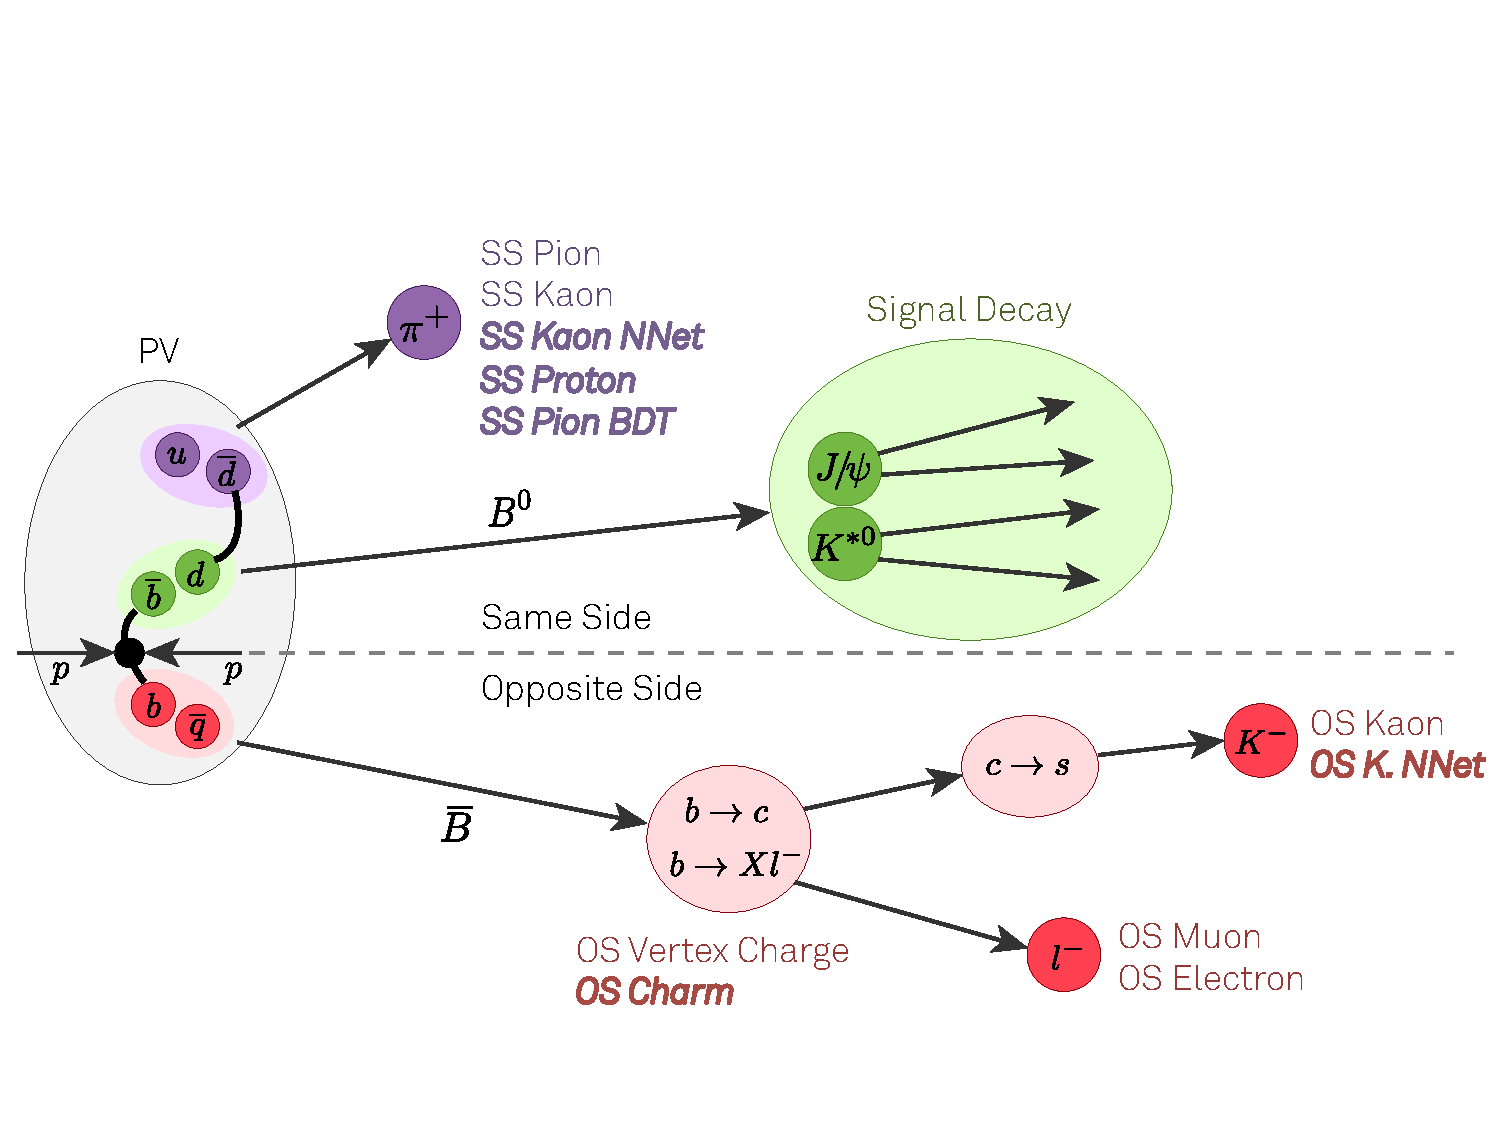
\includegraphics[width=\textwidth]{images/FlavourTaggingScheme.pdf}
    \caption{Track classification used in flavour tagging algorithms. \cite{ft_scheme}}
    \label{fig:ft_scheme}
\end{figure}


%\begin{table}
%    \centering
%    \caption{Listing of $B$-mesons and their quark contents.}
%    \begin{tabular}{c c c c | c c c c}
%        \toprule
%        \multicolumn{4}{c}{uncharged $B$-mesons} & \multicolumn{4}{c}{charged $B$-mesons} \\
%        \midrule
%        $B_d^0$ & $\bar{B}_d^0$ & $B_s^0$ & $\bar{B}_s^0$ & $B_u^-$ & $B_u^+$ & $B_c^-$ & $B_c^+$ \\
%        $b\bar{d}$ & $\bar{b}d$ & $b\bar{s}$ & $\bar{b}s$ & $b\bar{u}$ & $\bar{b}u$ & $b\bar{c}$ & $\bar{b}c$ \\
%        \bottomrule
%    \end{tabular}
%    \label{tab:B_mesons}
%\end{table}

%\begin{table}
%    \centering
%    \caption{Listing of $B$-mesons and their quark contents.}
%    \begin{tabular}{c c | c c}
%        \toprule
%        \multicolumn{2}{c}{uncharged $B$-mesons} & \multicolumn{2}{c}{charged $B$-mesons} \\
%        \midrule
%        $B^0 = b\bar{d}$ & $B_s^0 = b\bar{s}$ & $B^- = b\bar{u}$ & $B_c^- = b\bar{c}$ \\
%        $\bar{B}^0 = \bar{b}d$ & $\bar{B}_s^0 = \bar{b}s$ & $B^+ = \bar{b}u$ & $B_c^+ = \bar{b}c$ \\
%        \bottomrule
%    \end{tabular}
%    \label{tab:B_mesons}
%\end{table}

%\begin{align*}
%    \text{uncharged:} & B_d^0 = b\bar{d}, & \bar{B}_d^0 = \bar{b}d, & B_s^0 = b\bar{s}, & \bar{B}_s^0 = \bar{b}s \\
%    \text{charged:} & B_u^- = b\bar{u} & B_u^+ = \bar{b}u & B_c^- = b\bar{c} & B_c^+ = \bar{b}c
%\end{align*}



%The decay channels used in this thesis are
%\begin{align*}
%    B_d^0/\bar{B}_d^0 &\rightarrow J/\psi + K*^0 \, , \\
%    B_s^0/\bar{B}_s^0 &\rightarrow D_s^- + \pi^+ \, \text{and} \\
%    B_d^0/\bar{B}_d^0/B_s^0/\bar{B}_s^0 &\rightarrow J/\psi + K_S^0 \, .
%\end{align*}
\section{Classification algorithms} %TODO: Vukans corrections!

In general, classification algorithms are a type of supervised machine learning algorithms.
In machine learning, the parameters $\theta$ of a function $f$, also called a model, are optimized, so that predictions $\hat{y}=f(x|\theta)$ can be made that solves a given problem based on some input $x$.
Supervised machine learning is the optimization, also called training, of such models based on a dataset that contains the desired target $y$ for a given input. 
In classification algorithms, $y$ is a categorical variable and $\hat{y}$ can contain either discrete values or estimated probabilities. 
Therefore, classification algorithms try to assign a class to something (sample) based on measured quantities (features) that represent it. %TODO: "something" different word
For example, the main algorithm of this thesis evaluates the measured data of a $pp$-collision to estimate the class of the $B$ meson produced in this event.
The classification algorithms used in this thesis are described in the following sections.

\subsection{Boosted Decision Tree (BDT)}
\label{sec:BDT}

A Boosted Decision Tree (BDT) is an ensemble of multiple different decision trees trained and evaluated on the principles of gradient boosting.
Decision trees are binary trees with a decision condition at each node and a prediction score for each leaf.
The decisions are made on a single feature at each node.
The weighted sum of the prediction scores of all trees is then transformed using the logistic function to resemble a probability that the given sample belongs to one of the classes.
In gradient boosting the decision trees are trained iteratively, so that at each step the weighted sum of all previous decision trees and the current decision tree minimizes a given objective function.
To find the minimum, the gradient of the objective function with respect to the model parameters is calculated.
%All BDTs in this thesis are implemented in Python using the library XGBoost \cite{xgboost}.

\subsection{Neural Network (NN)}
\label{sec:NN}

\begin{figure}
    \centering
    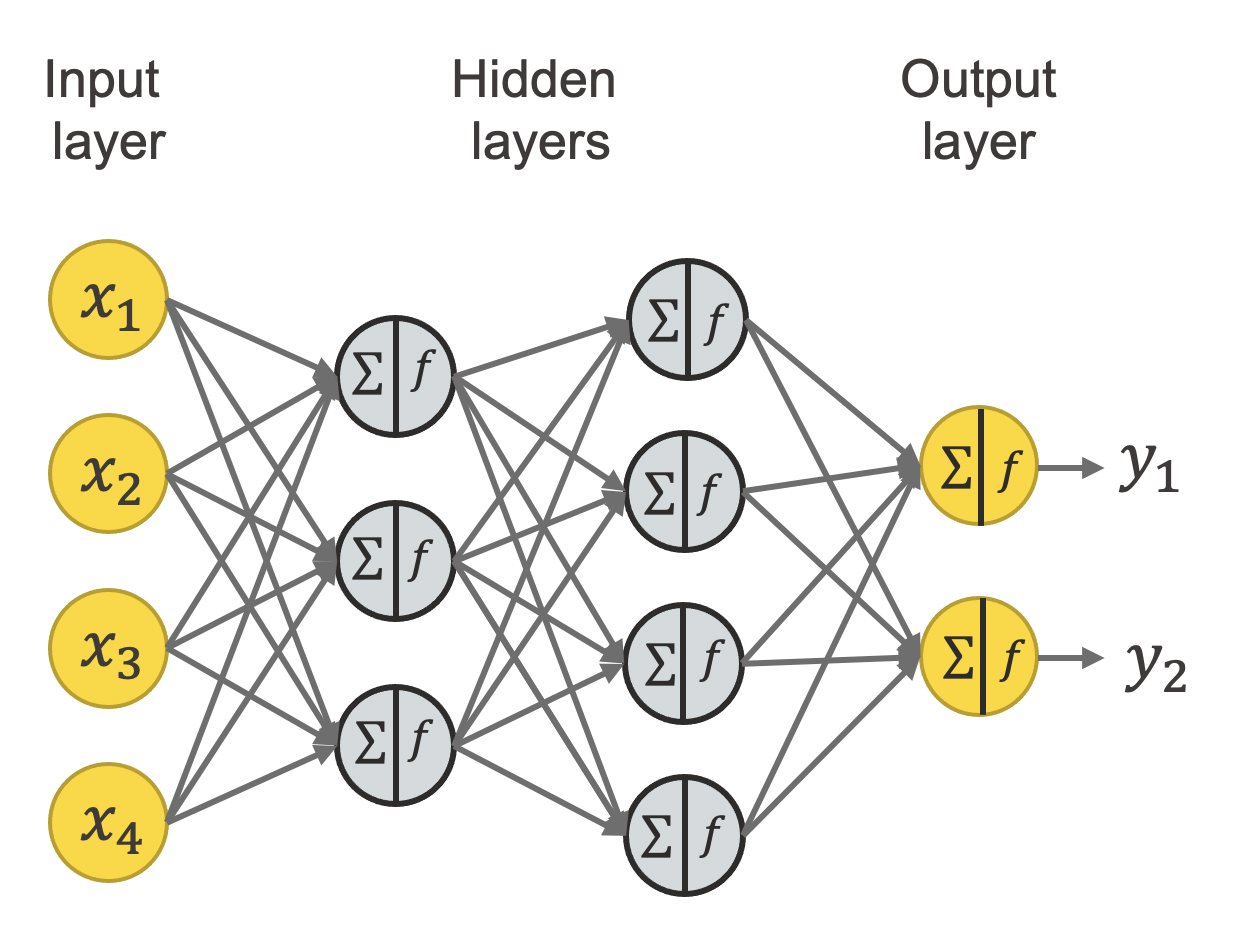
\includegraphics[width=0.5\textwidth]{images/NN_schematic.png}
    \caption{Example of a fully connected, feedforward neural network \cite{NN_schematic}.}
    \label{fig:NN_schematic}
\end{figure}

A Neural Network (NN) consists of multiple layers of (artificial) neurons to calculate an output vector $\hat{y}$ based on an input vector $x$.
The amount of layers and the amount of neurons per layer can be arbitrarily chosen based on the complexity of the problem.
\autoref{fig:NN_schematic} shows an example NN with 4 layers and is the basis of the following explanation.
Here, neurons are visualized as circles and represent a scalar number called activation $a$. 
The inputs of a neuron are marked by arrows from left to right and each arrow also represents a weight $w$.
The activation of each neuron is calculated by feeding the weighted sum 
\begin{equation*}
    z = \sum_{i \in \{\text{input neurons}\}} w_i \cdot a_i + b \, 
\end{equation*}
into a function $f(z)$ called the activation function.
$b$ is called the bias-weight of a neuron.
The activation functions used in this thesis are 
\begin{align*}
    f_\text{ReLU}(z) &= \max(0, z) \:\:\text{  and} \\
    f_\text{Sigmoid}(z) &= \frac{1}{1+e^{-z}} \, .
\end{align*}
The activations of the first layer are the values of $x$, and the activations of the last layer are used as the values of $\hat{y}$.
The layers in between the first and the last layer are called hidden layers.

To produce the desired outputs, the weights of a NN have to be adjusted in an iterative training process.
During the training process it is tried to find the minimum of a loss function that describes how well the NN solves the given problem based on the given target $y$.
Before the first iteration, all weights are initialized at random.
Each iteration then calculates the NN outputs and estimates the gradient of the loss function with respect to the weights.
Based on the gradient, the weights are adjusted towards the estimated minimum.
The step size at each iteration is determined by an optimizer algorithm.
This thesis uses the loss function binary cross entropy in combination with the optimizer Adam.
% TODO: bce formula and reference for Adam

NNs are prone to describe the training data too well, so that the model does not perform well on unseen data.
To prevent this overtraining, the regularization techniques used in this thesis are early stopping and dropout.

Early stopping calculates the loss on a validation dataset that is not used to adjust the weights.
If the loss does not improve for $N$ iterations the training is stopped and the weights of the best iteration based on this validation loss are used in the fitted NN.
This way, further adjusting of the NN to the training data is prevented and only the best results on the validation data are used.

In dropout, at each training iteration a random subset of neurons are disabled and only the remaining NN is evaluated and optimized.
Essentially, at each training iteration a smaller NN is trained and the co-dependence of neurons is reduced.
This makes the NN more robust and reduces overtraining.

\subsection{DeepSet}
\label{sec:DeepSet}

A DeepSet is an extension of NNs to allow inputs of sets of vectors.
DeepSets can therefore be used to solve problems where the data of each sample contains a variable length list and where the solution should be invariant under permutations of this list.
In this thesis, a DeepSet is used to classify $pp$-collision events that contain different amounts of tracks of which the order in the data should not matter.

The basic idea of DeepSets is that a function is invariant under permutations of the instances $x$ in a set $X$ if it can be written in the form 
\begin{equation*}
    f(X) = \rho \left( \sum_{x \in X} \phi (x) \right) \, .
\end{equation*}
This is also true, if the sum is replaced with any permutation invariant function.
In DeepSets $\rho$ and $\phi$ are represented by NNs and can be vector-valued \cite{deepset}.
In other words, a $\phi$-network first extracts some features about each instance in the set.
The feature values of all instances are then summed up and fed into a $\rho$-network that calculates the desired output.

The training of a DeepSet is fully analogous to the training of a NN.
The only difference is that a DeepSet consists of two NNs that are trained together.
%All DeepSets used in this thesis are implemented in Python using the library Pytorch \cite{pytorch}.




% A NN consists of multiple layers of (artificial) neurons to calculate an output vector $\hat{y}$ based on an input vector $x$.
% The amount of layers and the amount of neurons per layer can be arbitrarily chosen based on the complexity of the problem.
% A neuron represents a scalar number called activation that is calculated based on the weighted connections to the neurons of the previous % layer.
% The first layer of neurons is called the input layer and its activations are the values of $x$.


% A NN consists of multiple layers of (artificial) neurons to calculate an output vector $\hat{y}$ based on an input vector $x$.
% The amount of layers and the amount of neurons per layer can be arbitrarily chosen based on the complexity of the problem.
% A neuron calculates a scalar number called activation based on the activations of all neurons from the previous layer.
% The first layer of neurons is called the input layer and its activations are the values of $x$.
% When $a$ represents the activations of the previous layer, the linear activation of a single neuron in the next layer is
% \begin{equation*}
%     z = \sum_i w_i \cdot a_i + b \, .
% \end{equation*}
% $w_i$ is the weight associated with the connection to 
% 
% The activation of each other neuron is calculated through an activation function $f(z)$, where 
% \begin{equation*}
%     z = \sum_i w_i \cdot a_i + b \, .
% \end{equation*}
% $w_i$ is the weight of a connection between two neurons
% , the last layer is called the output layer and all layers in between are called hidden layers.
% 
% \autoref{fig:NN_schematic} shows an example NN with 4 layers.
% Each neuron is represented as a circle and the arrows represent the weighted connections between two neurons.
% 
% 
% A NN passes an input vector $x$ through multiple layers of (artificial) neurons to calculate an output vector $\hat{y}$ that may have a % different length than $x$.
% The amount of layers and the amount of neurons per layer can be arbitrarily chosen based on the complexity of the problem.
% A schematic of a NN with 3 layers is shown in \autoref{fig:NN_schematic}.
% Here, each neuron is represented by a circle and the arrows
% A neuron with an input vector $a$ first calculates a scalar 
% \begin{equation*}
%     z = \sum_i w_i \cdot a_i + b
% \end{equation*}
% called linear activation. 
% The vector $w$ and the scalar $b$ contain weights, that have to be optimized in the training process.
% Usually, this linear activation is then further transformed using an activation function.
% The activation functions used in this thesis are 
% \begin{align*}
%     \text{ReLU}(z) &= \max(0, z) & and \\
%     \text{Sigmoid}(z) &= \frac{1}{1+e^{-z}} \, .
% \end{align*}



\chapter{The LHCb detector}

The data used in this thesis originates from the LHCb detector, which is located at the LHC.
Therefore, this chapter first introduces the LHC and then describes the LHCb detector.

\section{The LHC}

The LHC (Large Hadron Collider) is a $\qty{27}{\km}$ long ring accelerator located in the vicinity of Geneva at the border of France and Switzerland. 
It is the largest particle accelerator in the world, and it is managed by CERN (European Organization for Nuclear Research).
The LHC can collide protons with a center-of-mass energy of up to $\qty{14}{\TeV}$ at a peak luminosity (interactions per area and time) of $\qty{e34}{\cm\squared\s}$ \cite{LHC}.
Additionally, the LHC can also accelerate heavy ions.
The four largest detectors at the LHC are ATLAS, CMS, ALICE and LHCb.
While ATLAS and CMS are general-purpose particle detectors, ALICE is dedicated to heavy ion collisions resulting in a quark-gluon plasma.

\section{The LHCb detector}

The LHCb detector is a particle detector dedicated to $pp$~collisions involving $c$ or $b$ quarks.
The goals of the LHCb collaboration are precision measurements of $C\!P$-violation and rare decays. 
To accomplish these goals, the LHCb detector has been build as a single arm forward-spectrometer covering angles to the beam pipe from $\qty{10}{\milli\radian}$ to $\qty{300}{\milli\radian}$ \cite{LHCb}. 
This design has been chosen because the majority of high energetic $b$-/$c$-hadron pairs, produced in $pp$~collisions, have Lorentz boosted velocities in the same direction as one of the incident protons.
An overview of the detector is shown in \cref{fig:lhcb_detector}.
The following paragraphs briefly describe the components of the LHCb detector based on the article \cite{LHCb}.

\begin{figure}
    \centering
    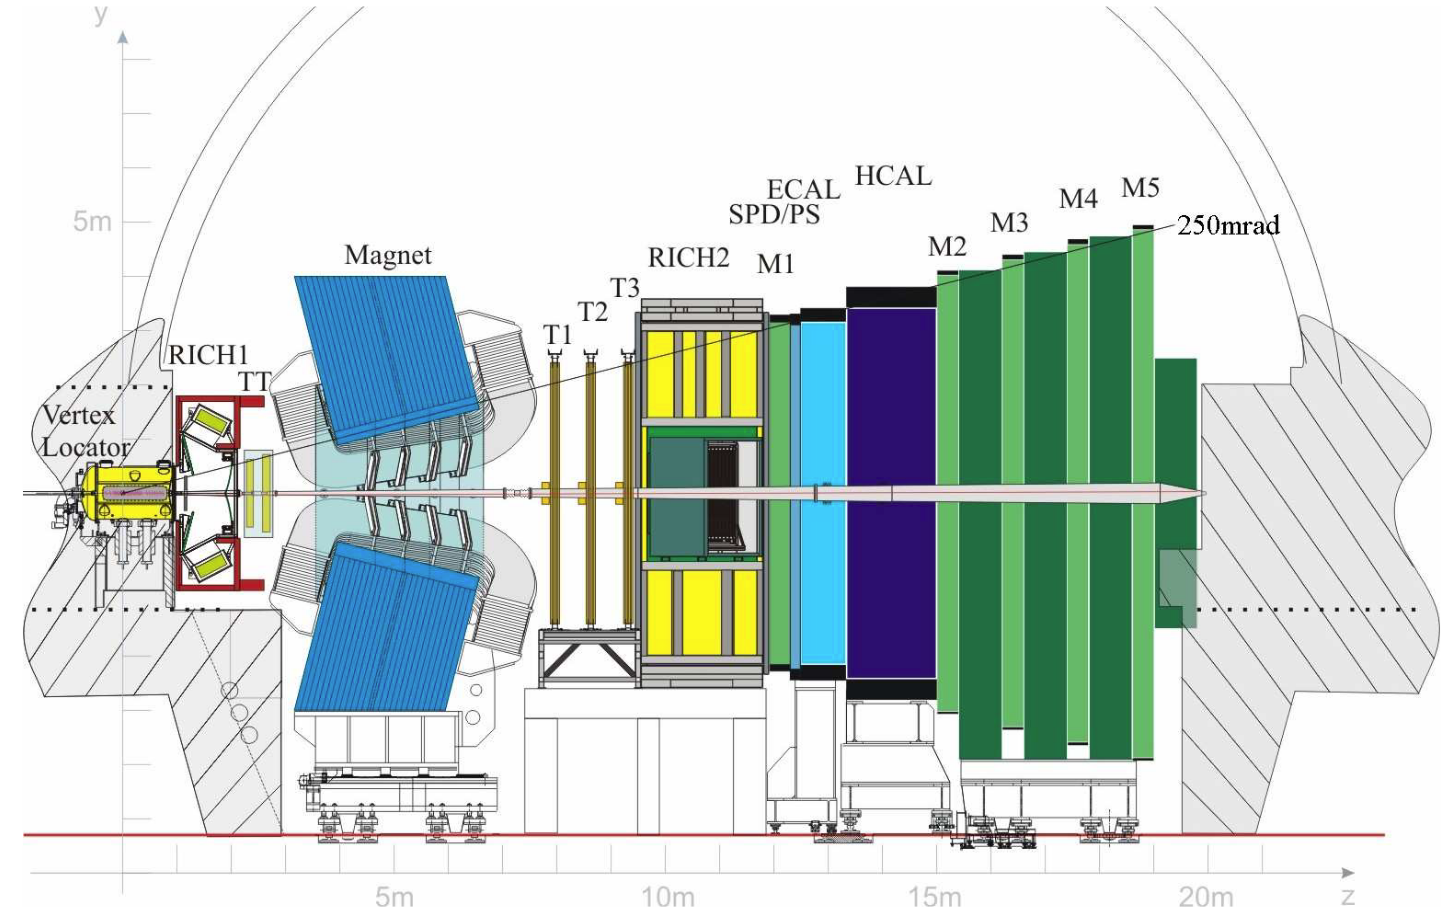
\includegraphics[width=\textwidth]{images/lhcb_detector.png}
    \caption{Sideview of the LHCb detector \cite{LHCb}. }
    \label{fig:lhcb_detector}
\end{figure}

A particle produced at the PV first traverses the Vertex Locator (VELO). 
There, the tracks of charged particles are measured using silicon semiconductor sensors at a resolution of about $\qty{4}{\micro\meter}$. 
This information then is primarily used to reconstruct the position of the primary and secondary vertices of the decay particles.

Beyond the VELO, the Tracking System then further measures the track points of the same particles. 
This is done in the Tracker Turicensis (TT) before the magnet and in the Trackers T1, T2 and T3 behind the magnet.
The dipole magnet bends the particle tracks through the Lorentz force so that the particle's momentum can be inferred.
While the TT and the inner parts of the T1-T3 also use silicon semiconductor sensors, the outer parts of the T1-T3 use straw-tube modules which are gaseous ionization detectors. 

The Ring Imaging Cherenkov detectors (RICH1, RICH2) are used to measure the particle velocities.
When charged particles traverse optically dense materials, the emission of Cherenkov radiation can be induced.
This radiation is then detected by photo multipliers. 
The opening angle of the emitted light cone is dependent on the velocity of the particle. 
The use of multiple radiators allows measuring particles with momenta between $\qty{1}{\GeV}$ and $\qty{100}{\GeV}$.
Comparing the momentum measured in the Tracking System with the velocity measured in the RICH detectors yields information particle's mass. 

The calorimeters (ECAL and HCAL) absorb and measure the energy of most particles.
In dense materials, particles can induce particle showers with the size directly related to the energy deposited.
Each calorimeter is structured in alternating layers of absorbers and scintillators. 
The electronic calorimeter~(ECAL) absorbs electrons, positrons and photons using lead, and the hadronic calorimeter~(HCAL) absorbs any hadrons using iron.
%The pad/preshower detector~(SPD/PS) reject $\pi$~background detected in the ECAL. 
The calorimeters are the only detectors at LHCb which can detect chargeless particles.

The muon chambers (M1-M5) track charged particles which pass through the calorimeters without absorption.
The majority of charged particles at this point in the detector are muons.
The iron layers between the muon chambers are used to absorb any non-muon particles.
M1-M5 are multi-wire proportional chambers to detect the track points of the muons.

The combined measured data of the RICH, the calorimeters and the muon chambers is used for particle identification.
Together with the Tracking System, this allows the reconstruction of the production and decay processes related to the $pp$-collision.

Due to the high precision of the LHCb detector, only a small portion of the $pp$-collisions visible in the LHCb detector can be permanently recorded for further analysis.
Therefore, a Trigger System is implemented to reduce the event detection rate from about $\qty{10}{\MHz}$ to about $\qty{2}{\kHz}$.
This system consists of the hardware trigger \enquote{Level-0}~(L0) and the software trigger \enquote{High Level Trigger}~(HLT).
The L0 collects information from the pile-up system of the VELO, the calorimeters and the muon chambers.
If the event does not contain particles with high transversal energy or momentum, it is rejected.
The L0 allows the readout of the whole detector at a rate of about $\qty{1}{\MHz}$.
The HLT then uses the data of all detector components to fully reconstruct the event and select events on various decision criteria.
At the final rate of about $\qty{2}{\kHz}$, the event data is permanently recorded and can then be accessed on demand by all members of the LHCb collaboration.

\chapter{Procedure and results}
\chapter{Conclusion}

In this thesis, a classification algorithm to distinguish $B_d$ from $B_s$ mesons in $pp$-collisions is developed, trained and evaluated.
This algorithm is intended to be independent of the signal $B$ decay channel and uses only data of the tracks associated with the signal $B$ meson without data of the signal decay.
For the training of supervised machine learning algorithms, simulated data of the decays $B_d \rightarrow J/\psi \, K^*$ and $B_s \rightarrow D^+_s \, \pi^-$ is used in this thesis. This data is based on simulations of the LHCb detector in the year 2016.

The developed algorithm first uses a Boosted Decision Tree (BDT) classifier to identify \enquote{same side} (SS) fragmentation tracks.
The SS fragmentation contains particles that are related to the $d\bar{d}$- or $s\bar{s}$-pair that is part of the production of the signal $B$. 
In contrast to other tracks in the data these SS tracks therefore contain relevant information for the distinction between $B_d$ and $B_s$ mesons.
Contained in the data are also tracks of the \enquote{opposite side} (OS) and tracks of particles unrelated to the signal $B$.
The OS contains particles related to the quark in the $b\bar{b}$-pair that is not in the signal $B$.
The output of this BDT is then used in a DeepSet classifier for the signal $B$.

Before training the final BDT, the available feature set is reduced.
To that end, a BDT is trained using all available features and features are then selected based on feature importance metrics called the gain and the permutation importance of the ROC AUC. The resulting 21 features, listed in \autoref{tab:SS_features}, are used by the final BDT.
After training the final BDT, the achieved separation between SS tracks and other tracks is evaluated using a ROC curve.
The ROC curve and the distribution of the BDT output are shown in \autoref{fig:SS_eval}. A ROC AUC of $0.763$ is achieved on test data.
Although the achieved separation is not sufficient to correctly identify most of the SS tracks, this BDT output can potentially help the DeepSet to form a decision.

For the feature selection of the DeepSet, the permutation importances of the accuracy and the ROC AUC are used.
This leads to the 23 features listed in \autoref{tab:B_features} that are used in the final DeepSet for the signal $B$ classification.
An indication that the BDT output ($\text{Prob}_\text{SS}$) has an impact on the DeepSet performance can be seen in \autoref{fig:B_importances}.
This however has to be interpreted with care, because feature importances can only be seen as estimates.
The trained DeepSet achieves a ROC AUC of $0.739$ on test data.
The ROC curve and the distribution of the DeepSet output are shown in \autoref{fig:B_eval}.

It can be seen that a clear separation of the $B$ mesons is achieved on simulated data.
However, any algorithm that has been developed using simulated data has to be tested on data that originates from actual measurements. 
Therefore, the developed algorithm of this thesis is tested on LHCb data of the decays $B_d \text{ or } B_s \rightarrow J/\psi \, K^0_\text{S}$.

Compared to the training data, LHCb data contains background events that do not actually involve $B_d$ or $B_s$ mesons.
Since evaluating the $B$ classification requires clearly visible $B_s$ peaks in the $B$ mass distribution, the number of background events has to be reduced beforehand.
This background reduction is done using a combination of manual cuts and a BDT that is trained on simulated data of the decay $B_d \rightarrow J/\psi \, K^0_\text{S}$.
This BDT achieves a ROC AUC of $0.989$ on test data.
The ROC curve achieved by the BDT and the total background reduction is shown in \autoref{fig:BKG_eval}.

The developed algorithm of this thesis is then applied to the background reduced data.
To evaluate the achieved separation, $B$ mass distributions with various selection criteria based on the DeepSet output ($\text{Prob}_{B_s}$) are used to fit a function.
The fit components that represent the combinatorial background, the $B_d$ peak and the $B_s$ peak are then integrated numerically.
This results in estimated counts of events attributed to the $B_d$ and $B_s$ mesons remaining after each selection.

The resulting ratios of the number of $B_s$ meson events over the number of $B_d$ meson events are shown in \autoref{fig:data_ratio}.
Here, selection criteria of the form $\text{Prob}_{B_s} \geq x$ show an upward trend with increasing $x$ values.
This could be an indication of some level of achieved separation between $B_s$ and $B_d$ mesons.
Selection criteria of the form $\text{Prob}_{B_s} \leq x$ show an increase of this ratio for lower $x$ values.
However, for small values of $x$ in $\text{Prob}_{B_s} \leq x$ there are too many combinatorial background events and an estimation of the $B_s$ peak is almost impossible. 
This is not the case for large values of $x$ in $\text{Prob}_{B_s} \geq x$ where a clear $B_s$ peak is visible.
All calculated ratios are compatible with the expected ratio for no achieved separation, but the upward trend for $\text{Prob}_{B_s} \geq x$ selections suggests at least a small achieved separation.

Another method to test the achieved separation is to plot the efficiencies of both the $B_d$ and $B_s$ mesons similar to a ROC curve.
This is shown in \autoref{fig:data_roc}.
Here, no clear signs of an achieved separation are visible.

Overall, the classification algorithm for separating Bs and Bd mesons was designed and tested on simulation and LHCb data. 
Unfortunately, the successful separation of $B_s$ and $B_d$ mesons on simulated data could not be reproduced on LHCb data.
Due to time constraints, further investigation into the reasons of this drastic performance loss is outside the scope of this thesis.
However, the achieved separation on simulated data is an indication that the strategy to use a DeepSet to distinguish $B_d$ from $B_s$ mesons based on data of the associated event could succeed.

%TODO: suggestions and weaknesses


%\appendix
% Hier beginnt der Anhang, nummeriert in lateinischen Buchstaben
%\chapter{Appendix} %TODO

Hier könnte ein Anhang stehen, falls Sie z.\,B.\ Code, Konstruktionszeichnungen oder Ähnliches mit in die Arbeit bringen wollen.
Im Normalfall stehen jedoch alle Ihre Resultate im Hauptteil der Bachelorarbeit und ein Anhang ist überflüssig.


\backmatter
\printbibliography

\chapter*{Danksagung} %TODO!


\cleardoublepage
% From https://www.tu-dortmund.de/studierende/im-studium/pruefungsangelegenheiten/allgemeine-vordrucke/
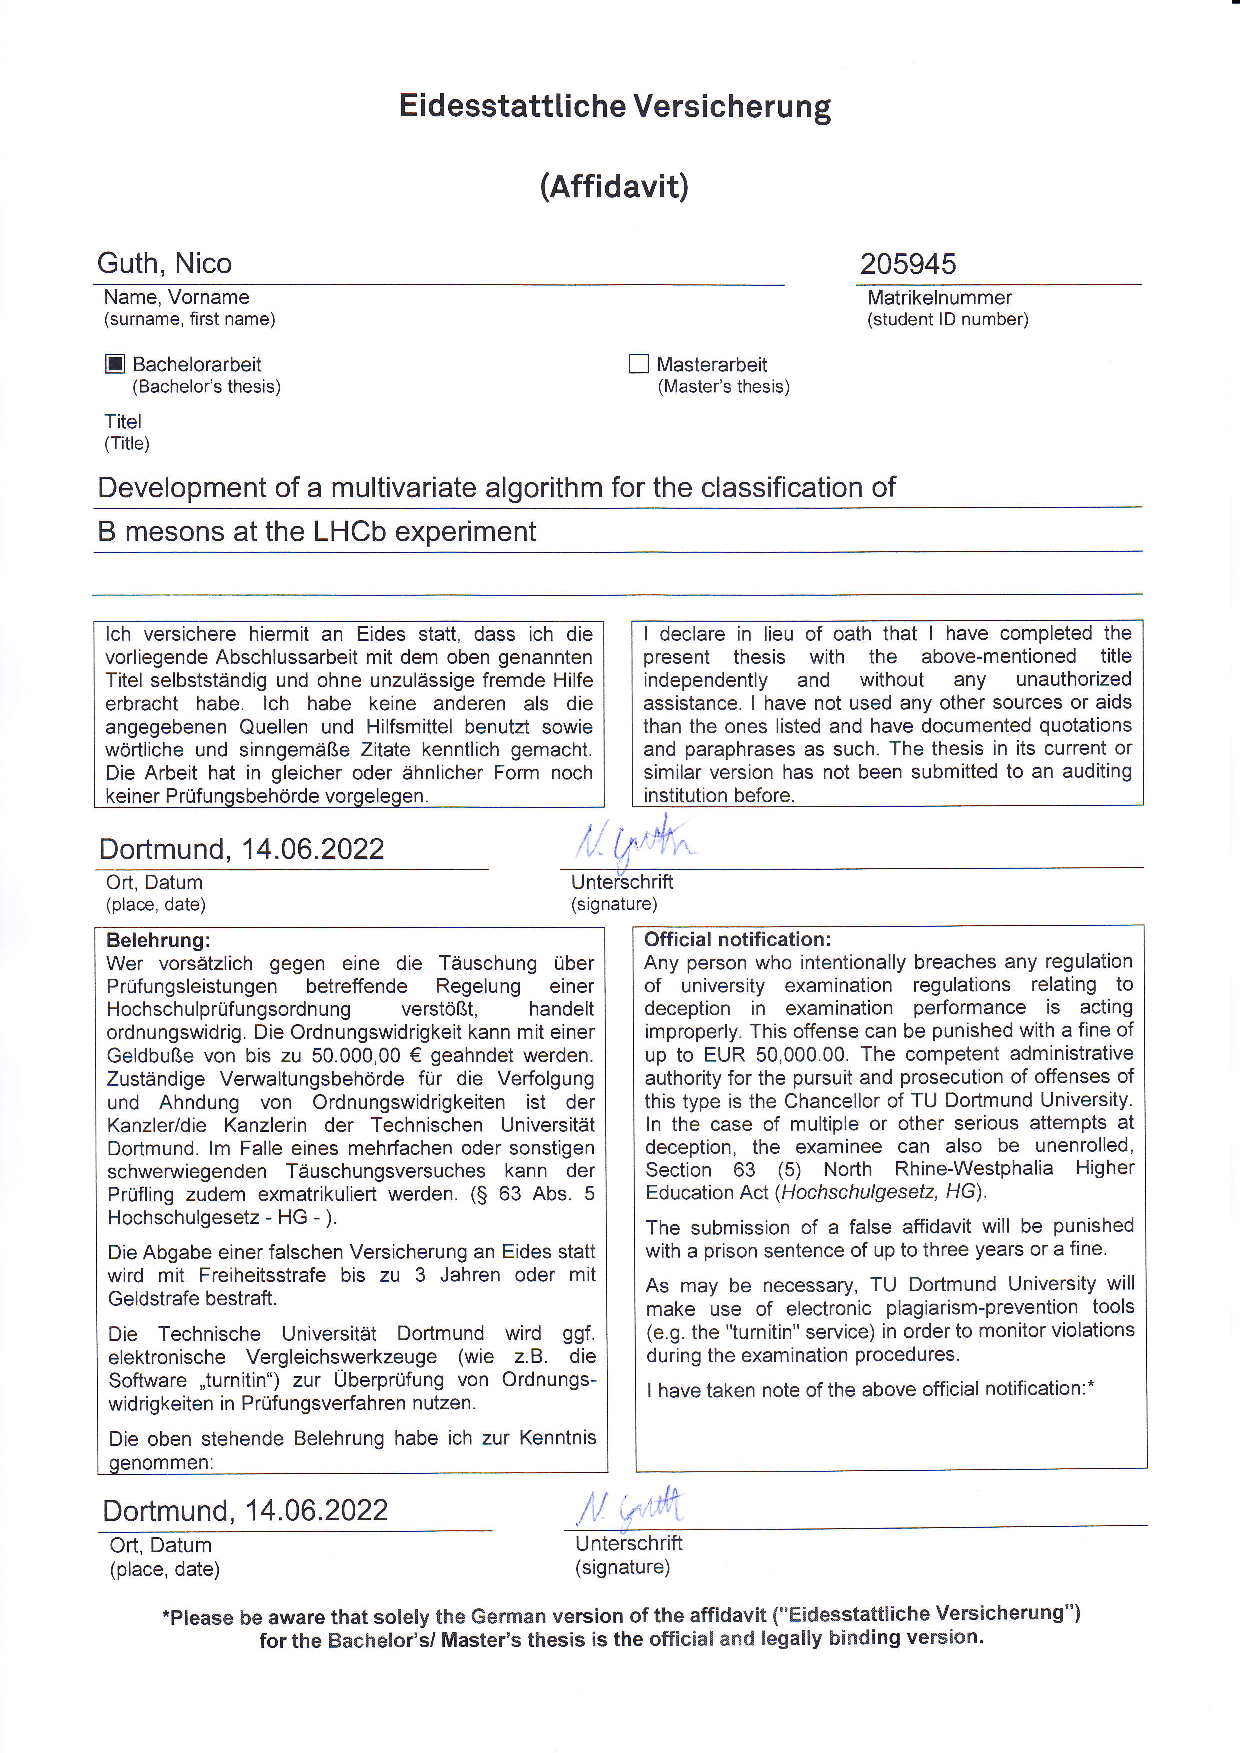
\includepdf{content/Eidesstattliche_Versicherung.pdf}

%\end{linenumbers}
\end{document}